\begin{chapterpage}{Probability}
  \chaptertitle{Probability}
  \label{probability}
  \label{ch_probability}
  \chaptersection{basicsOfProbability}
  \chaptersection{conditionalProbabilitySection}
  \chaptersection{smallPop}
  \chaptersection{randomVariablesSection}
  \chaptersection{contDist}
\end{chapterpage}
\renewcommand{\chapterfolder}{ch_probability}

\index{probability|(}

\chapterintro{Probability forms a foundation for statistics.
  and you're probably already familiar with many of the ideas.
  However, formalization of the concepts is new for most.
  This chapter aims to introduce probability concepts using
  many examples that will be familiar to most people. \\

  \noindent%
  While this chapter provides a theoretical foundation
  for the ideas introduced in later chapters,
  mastery of all concepts introduced in this chapter
  is not strictly required to understand or apply the
  methods introduced in the rest of this book.}

%  This chapter provides a theoretical foundation for
%  the ideas introduced in later chapters.
%  However, this chapter is not strictly required to
%  understand or apply the methods introduced in the
%  rest of this book.}




\section{Defining probability}
\label{basicsOfProbability}

Statistics is based on probability,
and while probability is not required for the applied
techniques in this book, it may help you gain a deeper
understanding of the methods and set a better foundation
for future courses.


\subsection{Introductory examples}

Before we get into technical ideas, let's walk through
some basic examples that may feel more familiar.

\begin{examplewrap}
\begin{nexample}{A ``die'', the singular of dice, is a cube with six faces numbered \resp{1}, \resp{2}, \resp{3}, \resp{4}, \resp{5}, and \resp{6}. What is the chance of getting \resp{1} when rolling a die?}\label{probOf1}
If the die is fair, then the chance of a \resp{1} is as good as the chance of any other number. Since there are six outcomes, the chance must be 1-in-6 or, equivalently, $1/6$.
\end{nexample}
\end{examplewrap}

\begin{examplewrap}
\begin{nexample}{What is the chance of getting a \resp{1} or \resp{2} in the next roll?}\label{probOf1Or2}
\resp{1} and \resp{2} constitute two of the six equally likely possible outcomes, so the chance of getting one of these two outcomes must be $2/6 = 1/3$.
\end{nexample}
\end{examplewrap}

\begin{examplewrap}
\begin{nexample}{What is the chance of getting either \resp{1}, \resp{2}, \resp{3}, \resp{4}, \resp{5}, or \resp{6} on the next roll?}\label{probOf123456}
100\%. The outcome must be one of these numbers.
\end{nexample}
\end{examplewrap}

\begin{examplewrap}
\begin{nexample}{What is the chance of not rolling a \resp{2}?}\label{probNot2}
Since the chance of rolling a \resp{2} is $1/6$ or $16.\bar{6}\%$, the chance of not rolling a \resp{2} must be $100\% - 16.\bar{6}\%=83.\bar{3}\%$ or $5/6$.

Alternatively, we could have noticed that not rolling a \resp{2} is the same as getting a \resp{1}, \resp{3}, \resp{4}, \resp{5}, or \resp{6}, which makes up five of the six equally likely outcomes and has probability $5/6$.
\end{nexample}
\end{examplewrap}

\begin{examplewrap}
\begin{nexample}{Consider rolling two dice. If $1/6$ of the time the first die is a \resp{1} and $1/6$ of those times the second die is a \resp{1}, what is the chance of getting two \resp{1}s?}\label{probOf2Ones}
If $16.\bar{6}$\% of the time the first die is a \resp{1} and $1/6$ of \emph{those} times the second die is also a \resp{1}, then the chance that both dice are \resp{1} is $(1/6)\times (1/6)$ or $1/36$.
\end{nexample}
\end{examplewrap}


\D{\newpage}

\subsection{Probability}

\index{random process|(}

We use probability to build tools to describe and understand apparent randomness. We often frame probability in terms of a \term{random process} giving rise to an \term{outcome}.
\begin{center}
\begin{tabular}{lll}
Roll a die &$\rightarrow$ & \resp{1}, \resp{2}, \resp{3}, \resp{4}, \resp{5}, or \resp{6} \\
Flip a coin &$\rightarrow$ & \resp{H} or \resp{T} \\
\end{tabular}
\end{center}
Rolling a die or flipping a coin is a seemingly random process and each gives rise to an outcome. 

\begin{onebox}{Probability}
The \term{probability} of an outcome is the proportion of times the outcome would occur if we observed the random process an infinite number of times.
\end{onebox}

Probability is defined as a proportion, and it always takes values between 0~and~1 (inclusively). It may also be displayed as a percentage between 0\% and 100\%.

Probability can be illustrated by rolling a die many times. Let $\hat{p}_n$ be the proportion of outcomes that are \resp{1} after the first $n$ rolls. As the number of rolls increases, $\hat{p}_n$ will converge to the probability of rolling a \resp{1}, $p = 1/6$. Figure~\ref{dieProp} shows this convergence for 100,000 die rolls. The tendency of $\hat{p}_n$ to stabilize around $p$ is described by the \term{Law of Large Numbers}. 

\begin{figure}[h]
\centering
\includegraphics[width=0.85\textwidth]{ch_probability/figures/dieProp/dieProp}
\caption{The fraction of die rolls that are 1 at each stage in a simulation. The proportion tends to get closer to the probability $1/6 \approx 0.167$ as the number of rolls increases.}
\label{dieProp}
\end{figure}

\begin{onebox}{Law of Large Numbers}
As more observations are collected, the proportion $\hat{p}_n$ of occurrences with a particular outcome converges to the probability $p$ of that outcome.
\end{onebox}

Occasionally the proportion will veer off from the probability and appear to defy the Law of Large Numbers, as $\hat{p}_n$ does many times in Figure~\ref{dieProp}. However, these deviations become smaller as the number of rolls increases.

Above we write $p$ as the probability of rolling a \resp{1}. We can also write this probability as
\begin{align*}
P(\text{rolling a \resp{1}})
\end{align*}
As we become more comfortable with this notation, we will abbreviate it further. For instance, if it is clear that the process is ``rolling a die'', we could abbreviate $P($rolling a \resp{1}$)$ as~$P($\resp{1}$)$. 

\begin{exercisewrap}
\begin{nexercise} \label{randomProcessExercise}
Random processes include rolling a die and flipping a coin. (a) Think of another random process. (b) Describe all the possible outcomes of that process. For instance, rolling a die is a random process with possible outcomes \mbox{\resp{1}, \resp{2}, ..., \resp{6}}.\footnotemark
\end{nexercise}
\end{exercisewrap}
\footnotetext{Here are four examples. (i) Whether someone gets sick in the next month or not is an apparently random process with outcomes \resp{sick} and \resp{not}. (ii) We can \emph{generate} a random process by randomly picking a person and measuring that person's height. The outcome of this process will be a positive number. (iii) Whether the stock market goes up or down next week is a seemingly random process with possible outcomes \resp{up}, \resp{down}, and \resp{no\us{}change}. Alternatively, we could have used the percent change in the stock market as a numerical outcome. (iv) Whether your roommate cleans her dishes tonight probably seems like a random process with possible outcomes \resp{cleans\us{}dishes} and \resp{leaves\us{}dishes}.}

What we think of as random processes are not necessarily random, but they may just be too difficult to understand exactly. The fourth example in the footnote solution to Guided Practice~\ref{randomProcessExercise} suggests a roommate's behavior is a random process. However, even if a roommate's behavior is not truly random, modeling her behavior as a random process can still be useful. 

%\begin{tipBox}{\tipBoxTitle{Modeling a process as random}
%It can be helpful to model a process as random even if it is not truly random.}
%\end{tipBox}

\index{random process|)}

\subsection{Disjoint or mutually exclusive outcomes}

\index{disjoint|(}
\index{mutually exclusive|(}

Two outcomes are called \term{disjoint} or \term{mutually exclusive} if they cannot both happen. For instance, if we roll a die, the outcomes \resp{1} and \resp{2} are disjoint since they cannot both occur. On the other hand, the outcomes \resp{1} and ``rolling an odd number'' are not disjoint since both occur if the outcome of the roll is a \resp{1}. The terms \emph{disjoint} and \emph{mutually exclusive} are equivalent and interchangeable.

Calculating the probability of disjoint outcomes is easy. When rolling a die, the outcomes \resp{1} and \resp{2} are disjoint, and we compute the probability that one of these outcomes will occur by adding their separate probabilities:
\begin{align*}
P(\text{\resp{1} or \resp{2}})
  = P(\text{\resp{1}})+P(\text{\resp{2}})
  = 1/6 + 1/6
  = 1/3
\end{align*}
What about  the probability of rolling a \resp{1}, \resp{2}, \resp{3}, \resp{4}, \resp{5}, or \resp{6}? Here again, all of the outcomes are disjoint so we add the probabilities:
\begin{align*}
&P(\text{\resp{1} or \resp{2} or \resp{3} or \resp{4}
    or \resp{5} or \resp{6}}) \\
  &\quad = P(\text{\resp{1}})+P(\text{\resp{2}})
      + P(\text{\resp{3}})+P(\text{\resp{4}})
      + P(\text{\resp{5}})+P(\text{\resp{6}}) \\
  &\quad = 1/6 + 1/6 + 1/6 + 1/6 + 1/6 + 1/6
  = 1
\end{align*}
The \term{Addition Rule} guarantees the accuracy of this approach when the outcomes are disjoint. 

\begin{onebox}{Addition Rule of disjoint outcomes}
  If $A_1$ and $A_2$ represent two disjoint outcomes,
  then the probability that one of them occurs is given by
  \begin{align*}
  P(A_1\text{ or } A_2) = P(A_1) + P(A_2)
  \end{align*}
  If there are many disjoint outcomes $A_1$, ..., $A_k$,
  then the probability that one of these outcomes will occur is
  \begin{align*}
  P(A_1) + P(A_2) + \cdots + P(A_k)
  \end{align*}
\end{onebox}

\D{\newpage}

\begin{exercisewrap}
\begin{nexercise}
We are interested in the probability of rolling a \resp{1}, \resp{4}, or \resp{5}. (a) Explain why the outcomes \resp{1}, \resp{4}, and \resp{5} are disjoint. (b) Apply the Addition Rule for disjoint outcomes to determine $P($\resp{1} or \resp{4} or \resp{5}$)$.\footnotemark
\end{nexercise}
\end{exercisewrap}
\footnotetext{(a) The random process is a die roll, and at most one of these outcomes can come up. This means they are disjoint outcomes. (b)~$P($\resp{1} or \resp{4} or \resp{5}$) = P($\resp{1}$)+P($\resp{4}$)+P($\resp{5}$) = \frac{1}{6} + \frac{1}{6} + \frac{1}{6} = \frac{3}{6} = \frac{1}{2}$}

\index{data!loans|(}
\begin{exercisewrap}
\begin{nexercise}
In the \data{loans} data set in Chapter~\ref{ch_summarizing_data},
the \var{homeownership} variable described whether the borrower
rents, has a mortgage, or owns her property.
Of the 10,000 borrowers, 3858 rented, 4789 had a mortgage,
and 1353 owned their home.\footnotemark{}
\begin{enumerate}[(a)]
\setlength{\itemsep}{0mm}
\item
    Are the outcomes \resp{rent}, \resp{mortgage},
    and \resp{own} disjoint?
\item
    Determine the proportion of loans with value \resp{mortgage}
    and \resp{own} separately.
\item
    Use the Addition Rule for disjoint outcomes to compute
    the probability a randomly selected loan from the data set
    is for someone who has a mortgage or owns her
    home.
\end{enumerate}
\end{nexercise}
\end{exercisewrap}
\footnotetext{(a)~Yes. Each loan is categorized in only one
level of \var{homeownership}.
(b)~Mortgage: $\frac{4789}{10000} = 0.479$.
Own: $\frac{1353}{10000} = 0.135$.
(c)~$P($\resp{mortgage} or \resp{own}$) = P($\resp{mortgage}$) + P($\resp{own}$) = 0.479 + 0.135 = 0.614$.}
\index{data!loans|)}

\index{event|(}

Data scientists rarely work with individual outcomes and instead consider \indexthis{\emph{sets}}{sets} or \indexthis{\emph{collections}}{collections} of outcomes. Let $A$ represent the event where a die roll results in \resp{1} or \resp{2} and $B$~represent the event that the die roll is a \resp{4} or a \resp{6}. We write $A$ as the set of outcomes $\{$\resp{1},~\resp{2}$\}$ and $B=\{$\resp{4}, \resp{6}$\}$. These sets are commonly called \termsub{events}{event}. Because $A$ and $B$ have no elements in common, they are disjoint events. $A$ and $B$ are represented in Figure~\ref{disjointSets}.

\begin{figure}[hhh]
  \centering
  \Figure{0.45}{disjointSets}
  \caption{Three events, $A$, $B$, and $D$, consist of
      outcomes from rolling a die.
      $A$ and $B$ are disjoint since they do not have
      any outcomes in common.}
  \label{disjointSets}
\end{figure}

The Addition Rule applies to both disjoint outcomes and disjoint events. The probability that one of the disjoint events $A$ or $B$ occurs is the sum of the separate probabilities:
\begin{align*}
P(A\text{ or }B) = P(A) + P(B) = 1/3 + 1/3 = 2/3
\end{align*}

\begin{exercisewrap}
\begin{nexercise}
(a) Verify the probability of event $A$, $P(A)$,
is $1/3$ using the Addition Rule.
(b)~Do the same for event $B$.\footnotemark
\end{nexercise}
\end{exercisewrap}
\footnotetext{(a)~$P(A) = P($\resp{1} or \resp{2}$)
    = P($\resp{1}$) + P($\resp{2}$)
    = \frac{1}{6} + \frac{1}{6}
    = \frac{2}{6}
    = \frac{1}{3}$.
    (b)~Similarly, $P(B) = 1/3$.}

\begin{exercisewrap}
\begin{nexercise} \label{exerExaminingDisjointSetsABD}
(a) Using Figure~\ref{disjointSets} as a reference, what outcomes are represented by event $D$? (b) Are events $B$ and $D$ disjoint? (c) Are events $A$ and $D$ disjoint?\footnotemark
\end{nexercise}
\end{exercisewrap}
\footnotetext{(a)~Outcomes \resp{2} and \resp{3}. (b)~Yes, events $B$ and $D$ are disjoint because they share no outcomes. (c)~The events $A$ and $D$ share an outcome in common, \resp{2}, and so are not disjoint.}

\begin{exercisewrap}
\begin{nexercise}
In Guided Practice~\ref{exerExaminingDisjointSetsABD}, you confirmed $B$ and $D$ from Figure~\ref{disjointSets} are disjoint. Compute the probability that event $B$ or event $D$~occurs.\footnotemark
\end{nexercise}
\end{exercisewrap}
\footnotetext{Since $B$ and $D$ are disjoint events, use the Addition Rule: $P(B$ or $D) = P(B) + P(D) = \frac{1}{3} + \frac{1}{3} = \frac{2}{3}$.}

\index{event|)}
\index{disjoint|)}
\index{mutually exclusive|)}


\D{\newpage}

\subsection{Probabilities when events are not disjoint}

Let's consider calculations for two events that are not disjoint in the context of a \indexthis{regular deck of 52 cards}{deck of cards}, represented in Figure~\ref{deckOfCards}. If you are unfamiliar with the cards in a regular deck, please see the footnote.\footnote{The 52 cards are split into four \term{suits}: $\clubsuit$ (club), {\color{redcards}$\diamondsuit$} (diamond), {\color{redcards}$\heartsuit$} (heart), $\spadesuit$ (spade). Each suit has its 13 cards labeled: \resp{2}, \resp{3}, ..., \resp{10}, \resp{J} (jack), \resp{Q} (queen), \resp{K} (king), and \resp{A} (ace). Thus, each card is a unique combination of a suit and a label, e.g. {\color{redcards}\resp{4$\heartsuit$}} and \resp{J$\clubsuit$}. The 12 cards represented by the jacks, queens, and kings are called \termsub{\resp{face cards}}{face card}. The cards that are {\color{redcards}$\diamondsuit$} or {\color{redcards}$\heartsuit$} are typically colored {\color{redcards}red} while the other two suits are typically colored black.}

\begin{figure}[h]
\centering
\begin{tabular}{lll lll lll lll l}
\resp{2$\clubsuit$} & \resp{3$\clubsuit$} & \resp{4$\clubsuit$} & \resp{5$\clubsuit$} & \resp{6$\clubsuit$} & \resp{7$\clubsuit$} & \resp{8$\clubsuit$} & \resp{9$\clubsuit$} & \resp{10$\clubsuit$} & \resp{J$\clubsuit$} & \resp{Q$\clubsuit$} & \resp{K$\clubsuit$} & \resp{A$\clubsuit$}  \\
\color{redcards} \resp{2$\diamondsuit$} & \color{redcards}\resp{3$\diamondsuit$} & \color{redcards}\resp{4$\diamondsuit$} & \color{redcards}\resp{5$\diamondsuit$} & \color{redcards}\resp{6$\diamondsuit$} & \color{redcards}\resp{7$\diamondsuit$} & \color{redcards}\resp{8$\diamondsuit$} & \color{redcards}\resp{9$\diamondsuit$} & \color{redcards}\resp{10$\diamondsuit$} & \color{redcards}\resp{J$\diamondsuit$} & \color{redcards}\resp{Q$\diamondsuit$} & \color{redcards}\resp{K$\diamondsuit$} & \color{redcards}\resp{A$\diamondsuit$} \\
\color{redcards}\resp{2$\heartsuit$} & \color{redcards}\resp{3$\heartsuit$} & \color{redcards}\resp{4$\heartsuit$} & \color{redcards}\resp{5$\heartsuit$} & \color{redcards}\resp{6$\heartsuit$} & \color{redcards}\resp{7$\heartsuit$} & \color{redcards}\resp{8$\heartsuit$} & \color{redcards}\resp{9$\heartsuit$} & \color{redcards}\resp{10$\heartsuit$} & \color{redcards}\resp{J$\heartsuit$} & \color{redcards}\resp{Q$\heartsuit$} & \color{redcards}\resp{K$\heartsuit$} & \color{redcards}\resp{A$\heartsuit$} \\
\resp{2$\spadesuit$} & \resp{3$\spadesuit$} & \resp{4$\spadesuit$} & \resp{5$\spadesuit$} & \resp{6$\spadesuit$} & \resp{7$\spadesuit$} & \resp{8$\spadesuit$} & \resp{9$\spadesuit$} & \resp{10$\spadesuit$} & \resp{J$\spadesuit$} & \resp{Q$\spadesuit$} & \resp{K$\spadesuit$} & \resp{A$\spadesuit$}
\end{tabular}
\caption{Representations of the 52 unique cards in a deck.}
\label{deckOfCards}
\end{figure}

\begin{exercisewrap}
\begin{nexercise}
(a) What is the probability that a randomly selected card is a diamond? (b)~What is the probability that a randomly selected card is a face card?\footnotemark
\end{nexercise}
\end{exercisewrap}
\footnotetext{(a) There are 52 cards and 13 diamonds. If the cards are thoroughly shuffled, each card has an equal chance of being drawn, so the probability that a randomly selected card is a diamond is $P({\color{redcards}\diamondsuit}) = \frac{13}{52} = 0.250$. (b)~Likewise, there are 12 face cards, so $P($face card$) = \frac{12}{52} = \frac{3}{13} = 0.231$.}

\term{Venn diagrams} are useful when outcomes can be categorized as ``in'' or ``out'' for two or three variables, attributes, or random processes. The Venn diagram in Figure~\ref{cardsDiamondFaceVenn} uses a circle to represent diamonds and another to represent face cards. If a card is both a diamond and a face card, it falls into the intersection of the circles. If it is a diamond but not a face card, it will be in part of the left circle that is not in the right circle (and so on). The total number of cards that are diamonds is given by the total number of cards in the diamonds circle: $10+3=13$. The probabilities are also shown (e.g. $10/52 = 0.1923$).

\begin{figure}
\centering
\includegraphics[width=0.65\textwidth]{ch_probability/figures/cardsDiamondFaceVenn/cardsDiamondFaceVenn}
\caption{A Venn diagram for diamonds and face cards.}
\label{cardsDiamondFaceVenn}
\end{figure}

Let $A$ represent the event that a randomly selected card is a diamond and $B$ represent the event that it is a face card. How do we compute $P(A$ or $B)$? Events $A$ and $B$ are not disjoint -- the cards {\color{redcards}$J\diamondsuit$}, {\color{redcards}$Q\diamondsuit$}, and {\color{redcards}$K\diamondsuit$} fall into both categories -- so we cannot use the Addition Rule for disjoint events. Instead we use the Venn diagram. We start by adding the probabilities of the two events:
\begin{align*}
P(A) + P(B)
  = P({\color{redcards}\diamondsuit}) + P(\text{face card})
  = 13/52 + 12/52
\end{align*}
However, the three cards that are in both events were counted twice, once in each probability. We must correct this double counting:
\begin{align*}
P(A\text{ or } B)
  &= P({\color{redcards}\diamondsuit}\text{ or face card}) \\
  &= P({\color{redcards}\diamondsuit}) + P(\text{face card})
      - P({\color{redcards}\diamondsuit}\text{ and face card}) \\
  &= 13/52 + 12/52 - 3/52 \\
  &= 22/52 = 11/26
\end{align*}
This equation is an example of the \term{General Addition Rule}. 

\begin{onebox}{General Addition Rule}
  If $A$ and $B$ are any two events, disjoint or not, then
  the probability that at least one of them will occur is
  \begin{align*}
  P(A\text{ or }B) = P(A) + P(B) - P(A\text{ and }B)
  \end{align*}
  where $P(A$ and $B)$ is the probability that both events occur.
\end{onebox}

\begin{tipBox}{\tipBoxTitle{``or'' is inclusive}
When we write ``or'' in statistics, we mean ``and/or'' unless we explicitly state otherwise. Thus, $A$ or $B$ occurs means $A$, $B$, or both $A$ and $B$ occur.}
\end{tipBox}

\begin{exercisewrap}
\begin{nexercise}
(a) If $A$ and $B$ are disjoint, describe why this implies $P(A$ and $B) = 0$. (b) Using part (a), verify that the General Addition Rule simplifies to the simpler Addition Rule for disjoint events if $A$ and $B$ are disjoint.\footnotemark
\end{nexercise}
\end{exercisewrap}
\footnotetext{(a) If $A$ and $B$ are disjoint, $A$ and $B$ can never occur simultaneously. (b) If $A$ and $B$ are disjoint, then the last $P(A\text{ and }B)$ term of in the General Addition Rule formula is 0 (see part (a)) and we are left with the Addition Rule for disjoint events.}

\index{data!loans|(}

\begin{exercisewrap}
\begin{nexercise}\label{emailSpamNumberVennExer}
% library(openintro); d <- loans_full_schema; table(d[,c("application_type", "homeownership")]); table(d[,c("application_type")]); table(d[,c("homeownership")])
In the \data{loans} data set describing 10,000 loans,
1495 loans were from joint applications
(e.g. a couple applied together),
4789 applicants had a mortgage,
and 950 had both of these characteristics.
Create a Venn diagram for this setup.\footnotemark
\end{nexercise}
\end{exercisewrap}
\footnotetext{%
  \begin{minipage}[t]{0.65\textwidth}
  Both the counts and corresponding {\color{oiB}probabilities}
  (e.g. $3839/10000 = 0.384$) are shown.
  Notice that the number of loans represented in the left
  circle corresponds to $3839 + 950 = 4789$, and the number
  represented in the right circle is $950 + 545 = 1495$.
  \end{minipage}\ %
  \begin{minipage}[c]{0.3\textwidth}
  \hfill\Figure{1.00}{loans_app_type_home_venn} \vspace{-13mm}
  \end{minipage}}

\begin{exercisewrap}
\begin{nexercise}
(a)~Use your Venn diagram from Guided Practice~\ref{emailSpamNumberVennExer} to determine the
probability a randomly drawn loan from the \data{loans}
data set is from a joint application where the couple had
a mortgage.
(b)~What is the probability that the loan had either of
these attributes?\footnotemark
\end{nexercise}
\end{exercisewrap}
\footnotetext{%
  (a)~The solution is represented by the intersection of
  the two circles: 0.095.
  (b)~This is the sum of the three disjoint probabilities shown
  in the circles: $0.384 + 0.095 + 0.055 = 0.534$
  (off by 0.001 due to a rounding error).}

\index{data!loans|)}


\D{\newpage}

\subsection{Probability distributions}

A \term{probability distribution} is a table of all disjoint outcomes and their associated probabilities. Figure~\ref{diceProb} shows the probability distribution for the sum of two dice. 

\begin{figure}[h] \small
\centering
\begin{tabular}{l ccc ccc ccc cc}
  \hline
  \ \vspace{-3mm} \\
Dice sum\vspace{0.3mm} & 2 & 3 & 4 & 5 & 6 & 7 & 8 & 9 & 10 & 11 & 12  \\
Probability & $\frac{1}{36}$ & $\frac{2}{36}$ & $\frac{3}{36}$ & $\frac{4}{36}$ & $\frac{5}{36}$ & $\frac{6}{36}$ & $\frac{5}{36}$ & $\frac{4}{36}$ & $\frac{3}{36}$ & $\frac{2}{36}$ & $\frac{1}{36}$\vspace{1mm} \\
   \hline
\end{tabular}
\caption{Probability distribution for the sum of two dice.}
\label{diceProb}
\end{figure}

\begin{onebox}{Rules for probability distributions}
A probability distribution is a list of the possible outcomes with corresponding probabilities that satisfies three rules: \vspace{-2mm}
\begin{enumerate}
\setlength{\itemsep}{0mm}
\item The outcomes listed must be disjoint.
\item Each probability must be between 0 and 1.
\item The probabilities must total 1. \vspace{1mm}
\end{enumerate}
\end{onebox}

\begin{exercisewrap}
\begin{nexercise}\label{usHouseholdIncomeDistsExercise}
Figure~\ref{usHouseholdIncomeDists} suggests three distributions for household income in the United States. Only one is correct. Which one must it be? What is wrong with the other two?\footnotemark
\end{nexercise}
\end{exercisewrap}
\footnotetext{The probabilities of (a) do not sum to~1.
    The second probability in (b) is negative.
    This leaves~(c), which sure enough satisfies the
    requirements of a distribution.
    One of the three was said to be the actual
    distribution of US household incomes,
    so it must be~(c).}

\begin{figure}
\centering
\begin{tabular}{r | cc cc}
  \hline
Income Range & \$0-25k & \$25k-50k & \$50k-100k & \$100k+ \\
  \hline
(a)\hspace{0.2mm}	 & 0.18 & 0.39 & 0.33 & 0.16 \\
(b)				 & 0.38 & -0.27 & 0.52 & 0.37 \\
(c)\hspace{0.2mm}	 & 0.28 & 0.27 & 0.29 & 0.16 \\
  \hline
\end{tabular}
\caption{Proposed distributions of US household incomes (Guided Practice~\ref{usHouseholdIncomeDistsExercise}).}
\label{usHouseholdIncomeDists}
\end{figure}

Chapter~\ref{introductionToData} emphasized the importance of plotting data to provide quick summaries. Probability distributions can also be summarized in a bar plot. For instance, the distribution of US household incomes is shown in Figure~\ref{usHouseholdIncomeDistBar} as a bar plot. %\footnote{It is also possible to construct a distribution plot when income is not artificially binned into four groups. \emph{Continuous} distributions are considered in Section~\ref{contDist}.}
The probability distribution for the sum of two dice is shown in Figure~\ref{diceProb} and plotted in Figure~\ref{diceSumDist}.

\begin{figure}[h]
  \centering
  \Figure{0.7}{usHouseholdIncomeDistBar}
  \caption{The probability distribution of US household income.}
  \label{usHouseholdIncomeDistBar}
\end{figure}

\begin{figure}
  \centering
  \Figure{0.73}{diceSumDist}
  \caption{The probability distribution of the sum of two dice.}
  \label{diceSumDist}
\end{figure}

In these bar plots, the bar heights represent the probabilities of outcomes. If the outcomes are numerical and discrete, it is usually (visually) convenient to make a bar plot that resembles a histogram, as in the case of the sum of two dice. Another example of plotting the bars at their respective locations is shown in Figure~\ref{bookCostDist} on page~\pageref{bookCostDist}.

\subsection{Complement of an event}

Rolling a die produces a value in the set $\{$\resp{1}, \resp{2}, \resp{3}, \resp{4}, \resp{5}, \resp{6}$\}$. This set of all possible outcomes is called the \term{sample space} ($S$)\index{S@$S$} for rolling a die. We often use the sample space to examine the scenario where an event does not occur.

Let $D=\{$\resp{2}, \resp{3}$\}$ represent the event that the outcome of a die roll is \resp{2} or \resp{3}. Then the \term{complement} of $D$ represents all outcomes in our sample space that are not in $D$, which is denoted by $D^c = \{$\resp{1}, \resp{4}, \resp{5}, \resp{6}$\}$. That is, $D^c$ is the set of all possible outcomes not already included in $D$. Figure~\ref{complementOfD} shows the relationship between $D$, $D^c$, and the sample space $S$. 

\begin{figure}[hht]
  \centering
  \Figure{0.55}{complementOfD}
  \caption{Event $D=\{$\resp{2}, \resp{3}$\}$ and its complement,
      $D^c = \{$\resp{1}, \resp{4}, \resp{5}, \resp{6}$\}$.
      $S$~represents the sample space, which is the set of
      all possible outcomes.}
  \label{complementOfD}
\end{figure}

\begin{exercisewrap}
\begin{nexercise}
(a) Compute $P(D^c) = P($rolling a \resp{1}, \resp{4}, \resp{5}, or \resp{6}$)$. (b) What is $P(D) + P(D^c)$?\footnotemark
\end{nexercise}
\end{exercisewrap}
\footnotetext{(a)~The outcomes are disjoint and each has probability $1/6$, so the total probability is $4/6=2/3$. (b)~We can also see that $P(D)=\frac{1}{6} + \frac{1}{6} = 1/3$. Since $D$ and $D^c$ are disjoint, $P(D) + P(D^c) = 1$.}

\begin{exercisewrap}
\begin{nexercise}
Events $A=\{$\resp{1}, \resp{2}$\}$ and $B=\{$\resp{4}, \resp{6}$\}$ are shown in Figure~\ref{disjointSets} on page~\pageref{disjointSets}. (a) Write out what $A^c$ and $B^c$ represent. (b)~Compute $P(A^c)$ and $P(B^c)$. (c)~Compute $P(A)+P(A^c)$ and $P(B)+P(B^c)$.\footnotemark
\end{nexercise}
\end{exercisewrap}
\footnotetext{Brief solutions: (a)~$A^c=\{$\resp{3}, \resp{4}, \resp{5}, \resp{6}$\}$ and $B^c=\{$\resp{1}, \resp{2}, \resp{3}, \resp{5}$\}$. (b)~Noting that each outcome is disjoint, add the individual outcome probabilities to get $P(A^c)=2/3$ and $P(B^c)=2/3$. (c)~$A$~and~$A^c$ are disjoint, and the same is true of $B$~and~$B^c$. Therefore, $P(A) + P(A^c) = 1$ and $P(B) + P(B^c) = 1$.}

A complement of an event $A$ is constructed to have two very important properties: (i) every possible outcome not in $A$ is in $A^c$, and (ii) $A$ and $A^c$ are disjoint. Property (i) implies
\begin{align*}
P(A\text{ or }A^c) = 1
\end{align*}
That is, if the outcome is not in $A$, it must be represented in $A^c$. We use the Addition Rule for disjoint events to apply Property (ii):
\begin{align*}
P(A\text{ or }A^c) = P(A) + P(A^c)
\end{align*}
Combining the last two equations yields a very useful
relationship between the probability of an event and
its complement.

\begin{onebox}{Complement}
  The complement of event $A$ is denoted $A^c$, and $A^c$
  represents all outcomes not in~$A$. $A$ and $A^c$ are
  mathematically related:
  \begin{align*}
  P(A) + P(A^c) = 1, \quad\text{i.e.}\quad P(A) = 1-P(A^c)
  \end{align*}
\end{onebox}

In simple examples, computing $A$ or $A^c$ is feasible in a few steps. However, using the complement can save a lot of time as problems grow in complexity.

\begin{exercisewrap}
\begin{nexercise}
Let $A$ represent the event where we roll two dice and their total is less than \resp{12}. (a)~What does the event $A^c$ represent? (b)~Determine $P(A^c)$ from Figure~\ref{diceProb} on page~\pageref{diceProb}. (c)~Determine $P(A)$.\footnotemark
\end{nexercise}
\end{exercisewrap}
\footnotetext{(a)~The complement of $A$: when the total is equal to \resp{12}. (b)~$P(A^c) = 1/36$. (c)~Use the probability of the complement from part (b), $P(A^c) = 1/36$, and the equation for the complement: $P($less than \resp{12}$) = 1 - P($\resp{12}$) = 1 - 1/36 = 35/36$.}

\begin{exercisewrap}
\begin{nexercise}
Find the following probabilities for rolling two dice:\footnotemark
\begin{enumerate}[(a)]
\setlength{\itemsep}{0mm}
\item The sum of the dice is \emph{not} \resp{6}. 
\item The sum is at least \resp{4}.
    That is, determine the probability of the event
    $B = \{$\resp{4}, \resp{5}, ..., \resp{12}$\}$.
\item The sum is no more than \resp{10}.
    That is, determine the probability of the event
    $D=\{$\resp{2}, \resp{3}, ..., \resp{10}$\}$.
\end{enumerate}
\end{nexercise}
\end{exercisewrap}
\footnotetext{(a)~First find $P($\resp{6}$)=5/36$, then use the complement: $P($not \resp{6}$) = 1 - P($\resp{6}$) = 31/36$.

(b)~First find  the complement, which requires much less effort: $P($\resp{2} or \resp{3}$)=1/36+2/36=1/12$. Then calculate $P(B) = 1-P(B^c) = 1-1/12 = 11/12$.

(c)~As before, finding the complement is the clever way to determine $P(D)$. First find $P(D^c) = P($\resp{11} or \resp{12}$)=2/36 + 1/36=1/12$. Then calculate $P(D) = 1 - P(D^c) = 11/12$.}


\subsection{Independence}
\label{probabilityIndependence}

Just as variables and observations can be independent, random processes can be independent, too. Two processes are \term{independent} if knowing the outcome of one provides no useful information about the outcome of the other. For instance, flipping a coin and rolling a die are two independent processes -- knowing the coin was heads does not help determine the outcome of a die roll. On the other hand, stock prices usually move up or down together, so they are not independent.

Example~\ref{probOf2Ones} provides a basic example of two independent processes: rolling two dice. We want to determine the probability that both will be \resp{1}. Suppose one of the dice is red and the other white. If the outcome of the red die is a \resp{1}, it provides no information about the outcome of the white die. We first encountered this same question in Example~\ref{probOf2Ones} (page~\pageref{probOf2Ones}), where we calculated the probability using the following reasoning: $1/6$ of the time the red die is a \resp{1}, and $1/6$ of \emph{those} times the white die will also be \resp{1}. This is illustrated in Figure~\ref{indepForRollingTwo1s}. Because the rolls are independent, the probabilities of the corresponding outcomes can be multiplied to get the final answer: $(1/6)\times(1/6)=1/36$. This can be generalized to many independent processes. 

\begin{figure}[hht]
\centering
\includegraphics[width=0.6\textwidth]{ch_probability/figures/indepForRollingTwo1s/indepForRollingTwo1s}
\caption{$1/6$ of the time, the first roll is a \resp{1}. Then $1/6$ of \emph{those} times, the second roll will also be a \resp{1}.}
\label{indepForRollingTwo1s}
\end{figure}

\begin{examplewrap}
\begin{nexample}{What if there was also a blue die independent of the other two? What is the probability of rolling the three dice and getting all \resp{1}s?}\label{threeDice}
The same logic applies from Example~\ref{probOf2Ones}. If $1/36$ of the time the white and red dice are both \resp{1}, then $1/6$ of \emph{those} times the blue die will also be \resp{1}, so multiply:
{\begin{align*}
P(white=\text{\small\resp{1} and } red=\text{\small\resp{1} and } blue=\text{\small\resp{1}})
	&= P(white=\text{\small\resp{1}})\times P(red=\text{\small\resp{1}})\times P(blue=\text{\small\resp{1}}) \\
	&= (1/6)\times (1/6)\times (1/6)
	= 1/216
\end{align*}} \vspace{-7mm}
\end{nexample}
\end{examplewrap}

Example~\ref{threeDice} illustrates what is called the Multiplication Rule for independent processes. 

\begin{onebox}{Multiplication Rule for independent processes}
  \index{Multiplication Rule|textbf}%
  If $A$ and $B$ represent events from two different and
  independent processes, then the probability that both $A$
  and $B$ occur can be calculated as the product of their
  separate probabilities:
  \begin{align*}
  P(A \text{ and }B) = P(A) \times  P(B)
  \end{align*}
  Similarly, if there are $k$ events $A_1$, ..., $A_k$
  from $k$ independent processes, then the probability
  they all occur is
  \begin{align*}
  P(A_1) \times  P(A_2)\times  \cdots \times  P(A_k)
  \end{align*}\vspace{-6mm}
\end{onebox}

\begin{exercisewrap}
\begin{nexercise} \label{ex2Handedness}
About 9\% of people are left-handed. Suppose 2 people are selected at random from the U.S. population. Because the sample size of 2 is very small relative to the population, it is reasonable to assume these two people are independent. (a)~What is the probability that both are left-handed? (b)~What is the probability that both are right-handed?\footnotemark
\end{nexercise}
\end{exercisewrap}
\footnotetext{(a) The probability the first person is left-handed is $0.09$, which is the same for the second person. We apply the Multiplication Rule for independent processes to determine the probability that both will be left-handed: $0.09\times 0.09 = 0.0081$.

(b) It is reasonable to assume the proportion of people who are ambidextrous (both right and left handed) is nearly 0, which results in $P($right-handed$)=1-0.09=0.91$. Using the same reasoning as in part~(a), the probability that both will be right-handed is $0.91\times 0.91 = 0.8281$.}

\begin{exercisewrap}
\begin{nexercise}
\label{ex5Handedness}%
Suppose 5 people are selected at random.\footnotemark\vspace{-1.5mm}
\begin{enumerate}
\setlength{\itemsep}{0mm}
\item[(a)] What is the probability that all are right-handed?
\item[(b)] What is the probability that all are left-handed?
\item[(c)] What is the probability that not all of the people are right-handed?
\end{enumerate}
\end{nexercise}
\end{exercisewrap}
\footnotetext{(a)~The abbreviations \resp{RH} and \resp{LH} are used for right-handed and left-handed, respectively. Since each are independent, we apply the Multiplication Rule for independent processes:
\begin{align*}
P(\text{all five are \resp{RH}})
&= P(\text{first = \resp{RH}, second = \resp{RH}, ..., fifth = \resp{RH}}) \\
&= P(\text{first = \resp{RH}})\times P(\text{second = \resp{RH}})\times  \dots \times P(\text{fifth = \resp{RH}}) \\
&= 0.91\times 0.91\times 0.91\times 0.91\times 0.91 = 0.624
\end{align*}

(b)~Using the same reasoning as in~(a), $0.09\times 0.09\times 0.09\times 0.09\times 0.09 = 0.0000059$

(c)~Use the complement, $P($all five are \resp{RH}$)$, to answer this question:
\begin{align*}
P(\text{not all \resp{RH}})
	= 1 - P(\text{all \resp{RH}})
	= 1 - 0.624 = 0.376
\end{align*}}

Suppose the variables \var{handedness} and
\var{sex} are independent,
i.e. knowing someone's \var{sex} provides no useful
information about their \var{handedness} and vice-versa.
Then we can compute whether a randomly selected person is
right-handed and female\footnote{The actual proportion of
  the U.S. population that is \resp{female} is about 50\%,
  and so we use 0.5 for the probability of sampling a woman.
  However, this probability does differ in other countries.}
using the Multiplication Rule:
\begin{align*}
P(\text{right-handed and female})
    &= P(\text{right-handed}) \times  P(\text{female}) \\
    &= 0.91 \times  0.50 = 0.455
\end{align*}


\begin{exercisewrap}
\begin{nexercise}
Three people are selected at random.\footnotemark \vspace{-1.5mm}
\begin{enumerate}
\setlength{\itemsep}{0mm}
\item[(a)] What is the probability that the first person is male and right-handed?
\item[(b)] What is the probability that the first two people are male and right-handed?.
\item[(c)] What is the probability that the third person is female and left-handed?
\item[(d)] What is the probability that the first two people are male and right-handed and the third person is female and left-handed?
\end{enumerate}
\end{nexercise}
\end{exercisewrap}
\footnotetext{Brief answers are provided. (a)~This can be written in probability notation as $P($a randomly selected person is male and right-handed$)=0.455$. (b)~0.207. (c)~0.045. (d)~0.0093.}

Sometimes we wonder if one outcome provides useful information about another outcome. The question we are asking is, are the occurrences of the two events independent? We say that two events $A$ and $B$ are independent if they satisfy
$P(A \text{ and }B) = P(A) \times  P(B)$.

\begin{examplewrap}
\begin{nexample}{If we shuffle up a deck of cards and draw one, is the event that the card is a heart independent of the event that the card is an ace?}
The probability the card is a heart is $1/4$ and the probability that it is an ace is $1/13$. The probability the card is the ace of hearts is $1/52$.
We check whether $P(A \text{ and }B) = P(A) \times  P(B)$
is satisfied:
\begin{align*}
P({\color{redcards}\heartsuit})\times P(\text{ace}) = \frac{1}{4}\times \frac{1}{13} = \frac{1}{52} 
					= P({\color{redcards}\heartsuit}\text{ and ace})
\end{align*}
Because the equation holds, the event that the card is a heart and the event that the card is an ace are independent events.
\end{nexample}
\end{examplewrap}


{\exercisesheader{}

% 1

\eoce{\qt{True or false\label{tf_prob_definitions}} Determine if the statements 
below are true or false, and explain your reasoning.
\begin{parts}
\item If a fair coin is tossed many times and the last eight tosses are all heads, 
then the chance that the next toss will be heads is somewhat less than 50\%.
\item Drawing a face card (jack, queen, or king) and drawing a red card from a 
full deck of playing cards are mutually exclusive events.
\item Drawing a face card and drawing an ace from a full deck of playing cards 
are mutually exclusive events.
\end{parts}
}{}

% 2

\eoce{\qt{Roulette wheel\label{roulette_wheel}} The game of roulette involves 
spinning a wheel with 38 slots: 18 red, 18 black, and 2 green. A ball is spun 
onto the wheel and will eventually land in a slot, where each slot has an equal 
chance of capturing the ball.

\noindent%
\begin{minipage}[c]{0.65\textwidth}
\raggedright\begin{parts}
\item You watch a roulette wheel spin 3 consecutive times and the ball lands on a 
red slot each time. What is the probability that the ball will land on a red slot 
on the next spin?
\item You watch a roulette wheel spin 300 consecutive times and the ball lands on 
a red slot each time. What is the probability that the ball will land on a red 
slot on the next spin?
\item Are you equally confident of your answers to parts~(a) and~(b)? Why or why 
not?
\end{parts}
\end{minipage}
\begin{minipage}[c]{0.05\textwidth}
\ 
\end{minipage}
\begin{minipage}[c]{0.28\textwidth}
\begin{center}
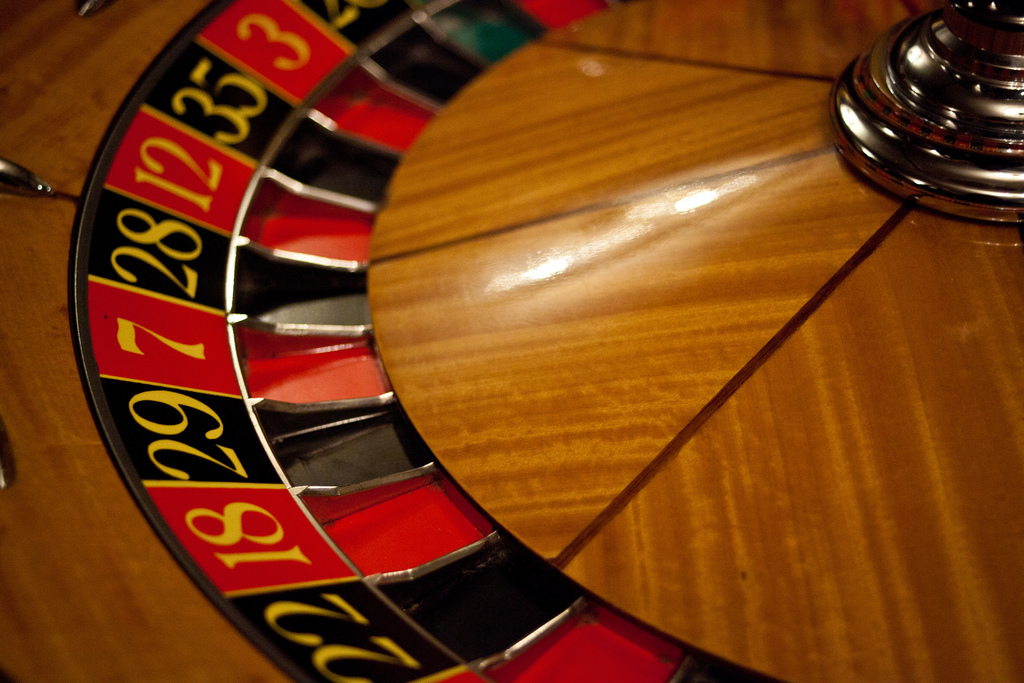
\includegraphics[width = \textwidth]{ch_probability/figures/eoce/roulette_wheel/roulette_wheel.jpg} \\
{\footnotesize Photo by H\r{a}kan Dahlstr\"{o}m \\
  (\oiRedirect{textbook-flickr_hakan_dahlstrom_roulette_wheel}{http://flic.kr/p/93fEzp}) \\
  \oiRedirect{textbook-CC_BY_2}{CC~BY~2.0~license}}
\end{center}
\end{minipage}
}{}

% 3

\eoce{\qt{Four games, one winner\label{four_games_one_winner}} Below are four 
versions of the same game. Your archnemesis gets to pick the version of the game, 
and then you get to choose how many times to flip a coin: 10 times or 100 times. 
Identify how many coin flips you should choose for each version of the game. It 
costs \$1 to play each game. Explain your reasoning.
\begin{parts}
\item If the proportion of heads is larger than 0.60, you win \$1.
\item If the proportion of heads is larger than 0.40, you win \$1.
\item If the proportion of heads is between 0.40 and 0.60, you win \$1.
\item If the proportion of heads is smaller than 0.30, you win \$1.
\end{parts}
}{}

% 4

\eoce{\qt{Backgammon\label{backgammon}} Backgammon is a board game for two 
players in which the playing pieces are moved according to the roll of two dice. 
Players win by removing all of their pieces from the board, so it is usually good 
to roll high numbers. You are playing backgammon with a friend and you roll two 
6s in your first roll and two 6s in your second roll. Your friend rolls two 3s in 
his first roll and again in his second row. Your friend claims that you are 
cheating, because rolling double 6s twice in a row is very unlikely. Using 
probability, show that your rolls were just as likely as~his.
}{}

% 5

\eoce{\qt{Coin flips\label{coin_flips}} If you flip a fair coin 10 times, what is 
the probability of
\begin{parts}
\item getting all tails? 
\item getting all heads? 
\item getting at least one tails? 
\end{parts}
}{}

% 6

\eoce{\qt{Dice rolls\label{dice_rolls}} If you roll a pair of fair dice, what is 
the probability of
\begin{parts}
\item getting a sum of 1?
\item getting a sum of 5?
\item getting a sum of 12?
\end{parts}
}{}

\D{\newpage}

% 7

\eoce{\qt{Swing voters\label{swing_voters}} A Pew Research survey asked 2,373 
randomly sampled registered voters their political affiliation (Republican, 
Democrat, or Independent) and whether or not they identify as swing voters. 35\% 
of respondents identified as Independent, 23\% identified as swing voters, and 
11\% identified as both.\footfullcite{indepSwing}
\begin{parts}
\item Are being Independent and being a swing voter disjoint, i.e. mutually 
exclusive?
\item Draw a Venn diagram summarizing the variables and their associated 
probabilities.
\item What percent of voters are Independent but not swing voters?
\item What percent of voters are Independent or swing voters?
\item What percent of voters are neither Independent nor swing voters?
\item Is the event that someone is a swing voter independent of the event that 
someone is a political Independent?
\end{parts}
}{}

% 8

\eoce{\qt{Poverty and language\label{poverty_language}} The American Community 
Survey is an ongoing survey that provides data every year to give communities the 
current information they need to plan investments and services. The 2010 American 
Community Survey estimates that 14.6\% of Americans live below the poverty line, 
20.7\% speak a language other than English (foreign language) at home, and 4.2\% 
fall into both categories. \footfullcite{poorLang}
\begin{parts}
\item Are living below the poverty line and speaking a foreign language at home 
disjoint?
\item Draw a Venn diagram summarizing the variables and their associated 
probabilities.
\item What percent of Americans live below the poverty line and only speak 
English at home?
\item What percent of Americans live below the poverty line or speak a foreign 
language at home?
\item What percent of Americans live above the poverty line and only speak 
English at home? 
\item Is the event that someone lives below the poverty line independent of the 
event that the person speaks a foreign language at home?
\end{parts}
}{}

% 9

\eoce{\qt{Disjoint vs. independent\label{disjoint_indep}} In parts~(a) and~(b), 
identify whether the events are disjoint, independent, or neither (events cannot 
be both disjoint and independent).
\begin{parts}
\item You and a randomly selected student from your class both earn A's in this 
course. 
\item You and your class study partner both earn A's in this course.
\item If two events can occur at the same time, must they be dependent?
\end{parts}
}{}

% 10

\eoce{\qt{Guessing on an exam\label{guessing_on_exam}} In a multiple choice exam, 
there are 5 questions and 4 choices for each question (a, b, c, d). Nancy has not 
studied for the exam at all and decides to randomly guess the answers. What is 
the probability that:
\begin{parts}
\item the first question she gets right is the $5^{th}$ question?
\item she gets all of the questions right?
\item she gets at least one question right?
\end{parts}
}{}

\D{\newpage}

% 11

\eoce{\qt{Educational attainment of couples\label{edu_attain_couples}} The table 
below shows the distribution of education level attained by US residents by 
gender based on data collected in the 2010 American Community Survey.
\footfullcite{eduSex}
\begin{center}
\begin{tabular}{l p{7cm} c c }
&                                       & \multicolumn{2}{c}{\textit{Gender}} \\
\cline{3-4}
&                                                   & Male  & Female \\
\cline{2-4}
& Less than 9th grade                               & 0.07  & 0.13 \\
& 9th to 12th grade, no diploma                     & 0.10  & 0.09 \\
\textit{Highest}    & HS graduate (or equivalent)   & 0.30  & 0.20 \\
\textit{education}  & Some college, no degree       & 0.22  & 0.24 \\ 
\textit{attained}   & Associate's degree            & 0.06  & 0.08 \\
& Bachelor's degree                                 & 0.16  & 0.17 \\
& Graduate or professional degree                   & 0.09  & 0.09 \\
\cline{2-4} 
& Total                                             & 1.00  & 1.00
\end{tabular}
\end{center}
\begin{parts}
\item What is the probability that a randomly chosen man has at least a 
Bachelor's degree?
\item What is the probability that a randomly chosen woman has at least a 
Bachelor's degree?
\item What is the probability that a man and a woman getting married both have at 
least a Bachelor's degree? Note any assumptions you must make to answer this 
question.
\item If you made an assumption in part~(c), do you think it was reasonable? If 
you didn't make an assumption, double check your earlier answer and then return 
to this part.
\end{parts}
}{}

% 12

\eoce{\qt{School absences\label{school_absences}} Data collected at elementary 
schools in DeKalb County, GA suggest that each year roughly 25\% of students miss 
exactly one day of school, 15\% miss 2 days, and 28\% miss 3 or more days due to 
sickness. \footfullcite{Mizan:2011}
\begin{parts}
\item What is the probability that a student chosen at random doesn't miss any 
days of school due to sickness this year?
\item What is the probability that a student chosen at random misses no more than 
one day?
\item What is the probability that a student chosen at random misses at least one 
day?
\item If a parent has two kids at a DeKalb County elementary school, what is the 
probability that neither kid will miss any school? Note any assumption you must 
make to answer this question.
\item If a parent has two kids at a DeKalb County elementary school, what is the 
probability that both kids will miss some school, i.e. at least one day? Note any 
assumption you make.
\item If you made an assumption in part~(d) or~(e), do you think it was 
reasonable? If you didn't make any assumptions, double check your earlier answers.
\end{parts}
}{}
}




%_________________
\section{Conditional probability}
\label{conditionalProbabilitySection}

There can be rich relationships between two or more
variables that are useful to understand.
For example a car insurance company will consider
information about a person's driving history to assess
the risk that they will be responsible for an accident.
These types of relationships are the realm of conditional
probabilities.


\subsection{Exploring probabilities with a contingency table}

\index{data!photo\_classify|(}

\newcommand{\fashN}{1822}
% In order of ML, then Human
\newcommand{\fashYY}{197}
\newcommand{\fashYN}{22}
\newcommand{\fashYA}{219}
\newcommand{\fashNY}{112}
\newcommand{\fashNN}{1491}
\newcommand{\fashNA}{1603}
\newcommand{\fashAY}{309}
\newcommand{\fashAN}{1513}
\newcommand{\fashAA}{\fashN{}}
%\newcommand{\fashPYY}{}
%\newcommand{\fashPYN}{}
%\newcommand{\fashPNY}{}
%\newcommand{\fashPNN}{}
%\newcommand{\fashPYA}{0.12}
%\newcommand{\fashPNA}{0.88}
%\newcommand{\fashPAY}{}
%\newcommand{\fashPAN}{}
%\newcommand{\fashPYCY}{}
%\newcommand{\fashPYCN}{}
%\newcommand{\fashPNCY}{}
%\newcommand{\fashPNCN}{}
\newcommand{\fashCYPY}{0.96}
\newcommand{\fashCYPN}{0.04}
\newcommand{\fashCNPY}{0.07}
\newcommand{\fashCNPN}{0.93}

The \data{photo\us{}classify} data set represents
a classifier a sample of \fashN{} photos from photo sharing website.
Data scientists have been working to improve a classifier for
whether the photo is about fashion or not, and these 659 photos
represent a test for their classifier.
Each photo gets two classifications:
the first is called \var{mach\us{}learn} and gives
a classification from a machine
learning~(ML)\index{machine learning (ML)} system of
either \resp{pred\us{}fashion} or \resp{pred\us{}not}.
Each of these \fashN{} photos have also been classified carefully
by a team of people, which we take to be the source of truth;
this variable is called \var{truth} and takes values
\resp{fashion} and \resp{not}.
Figure~\ref{contTableOfFashionPhotos} summarizes the results.

\begin{figure}[ht]
\centering
\begin{tabular}{ll ccc rr}
&& \multicolumn{2}{c}{\var{truth}} & \hspace{1cm} &  \\
\cline{3-4}
&& \resp{fashion} & \resp{not} & Total  \\
\cline{2-5}
& \resp{pred\us{}fashion} &
    \fashYY{} & \fashYN{} & \fashYA{} \\
\raisebox{1.5ex}[0pt]{\var{pred\us{}not}}
    & \resp{not} \hspace{0.5cm} &
    \fashNY{} & \fashNN{} & \fashNA{}   \\
\cline{2-5}
& Total & \fashAY{} & \fashAN{} & \fashN{} \\
\end{tabular}
\caption{Contingency table summarizing the
    \data{photo\us{}classify} data set.}
\label{contTableOfFashionPhotos}
\end{figure}
% library(openintro); table(photo_classify)

\begin{figure}[ht]
  \centering
  \Figure{0.65}{photoClassifyVenn}
  \caption{A Venn diagram using boxes for the
      \data{photo\us{}classify} data set.}
  \label{photoClassifyVenn}
\end{figure}

\begin{examplewrap}
\begin{nexample}{If a photo is actually about fashion,
    what is the chance the ML classifier correctly identified
    the photo as being about fashion?}
  We can estimate this probability using the data.
  Of the \fashAY{} fashion photos,
  the ML algorithm correctly classified \fashYY{} of the photos:
\begin{align*}
P(\text{\var{mach\us{}learn} is \resp{pred\us{}fashion}
    given \var{truth} is \resp{fashion}})
  = \frac{\fashYY{}}{\fashAY{}}
  = 0.638
\end{align*}
\end{nexample}
\end{examplewrap}

\begin{examplewrap}
\begin{nexample}{We sample a photo from the data set
    and learn the ML algorithm predicted this photo
    was not about fashion.
    What is the probability that it was incorrect and
    the photo is about fashion?}
  If the ML classifier suggests a photo is not about fashion,
  then it comes from the second row in the data set.
  Of~these \fashNA{} photos, \fashNY{} were actually
  about fashion:
\begin{align*}
P(\text{\var{truth} is \resp{fashion}
    given \var{mach\us{}learn} is \resp{pred\us{}not}})
  = \frac{\fashNY{}}{\fashNA{}}
  = 0.070
\end{align*}
\end{nexample}
\end{examplewrap}

\subsection{Marginal and joint probabilities}
\label{marginalAndJointProbabilities}

\index{marginal probability|(}
\index{joint probability|(}

Figure~\ref{contTableOfFashionPhotos} includes row and
column totals for each variable separately in the
\data{photo\us{}classify} data set.
These totals represent
\termsub{marginal probabilities}{marginal probability}
for the sample, which are the probabilities based on a
single variable without regard to any other variables.
For instance, a probability based solely on the
\var{mach\us{}learn} variable is a marginal probability:
\begin{align*}
P(\text{\var{mach\us{}learn} is \resp{pred\us{}fashion}})
    = \frac{\fashYA{}}{\fashN{}}
    = 0.12
\end{align*}
A probability of outcomes for two or more variables
or processes is called a
\termsub{joint \mbox{probability}}{joint probability}:
\begin{align*}
P(\text{\var{mach\us{}learn} is \resp{pred\us{}fashion}
    and \var{truth} is \resp{fashion}})
  = \frac{\fashYY{}}{\fashN{}}
  = 0.11
\end{align*}
It is common to substitute a comma for ``and'' in a joint
probability, although using either the word ``and'' or a
comma is acceptable:
\begin{center}
$P(\text{\var{mach\us{}learn} is \resp{pred\us{}fashion},
    \var{truth} is \resp{fashion}})$ \\[2mm]
means the same thing as \\[2mm]
$P(\text{\var{mach\us{}learn} is \resp{pred\us{}fashion}
    and \var{truth} is \resp{fashion}})$
\end{center}

\begin{onebox}{Marginal and joint probabilities}
  If a probability is based on a single variable,
  it is a \emph{\hiddenterm{marginal probability}}.
  The probability of outcomes for two or more variables
  or processes is called a \emph{\hiddenterm{joint probability}}.
\end{onebox}

We use \term{table proportions} to summarize joint probabilities
for the \data{photo\us{}classify} sample.
These proportions are computed by dividing each count in
Figure~\ref{contTableOfFashionPhotos} by the table's total,
\fashN{}, to obtain the proportions in
Figure~\ref{photoClassifyProbTable}.
The joint probability distribution of the \var{mach\us{}learn}
and \var{truth} variables is shown in
Figure~\ref{photoClassifyDistribution}.

\begin{figure}[h]
\centering
\begin{tabular}{l rr r}
\hline
& \var{truth}: \resp{fashion} &
    \var{truth}: \resp{not} & Total  \\
\hline
\var{mach\us{}learn}: \resp{pred\us{}fashion} \hspace{0.5cm}
    & 0.1081 & 0.0121 & 0.1202 \\
\var{mach\us{}learn}: \resp{pred\us{}not}
    & 0.0615 & 0.8183 & 0.8798  \\
\hline
Total & 0.1696 & 0.8304 & 1.00 \\
\hline
\end{tabular}
\caption{Probability table summarizing the
    \var{photo\us{}classify} data set.}
\label{photoClassifyProbTable}
\end{figure}

\begin{figure}[h]
\centering
\begin{tabular}{l c}
  \hline
Joint outcome & Probability \\
  \hline
\var{mach\us{}learn} is \resp{pred\us{}fashion}
    and \var{truth} is \resp{fashion} & 0.1081 \\
\var{mach\us{}learn} is \resp{pred\us{}fashion}
    and \var{truth} is \resp{not} & 0.0121 \\
\var{mach\us{}learn} is \resp{pred\us{}not}
    and \var{truth} is \resp{fashion} & 0.0615 \\
\var{mach\us{}learn} is \resp{pred\us{}not}
    and \var{truth} is \resp{not} & 0.8183 \\
   \hline
Total & 1.0000 \\
\hline
\end{tabular}
\caption{Joint probability distribution for the \data{photo\us{}classify} data set.}
\label{photoClassifyDistribution}
\end{figure}

\D{\newpage}

\begin{exercisewrap}
\begin{nexercise}
Verify Figure~\ref{photoClassifyDistribution} represents
a probability distribution: events are disjoint,
all probabilities are non-negative, and the probabilities
sum to~1.\footnotemark
\end{nexercise}
\end{exercisewrap}
\footnotetext{Each of the four outcome combination are disjoint,
   all probabilities are indeed non-negative, and the sum of
   the probabilities is $0.1081 + 0.0121 + 0.0615 + 0.8183 = 1.00$.}

We can compute marginal probabilities using joint probabilities
in simple cases.
For example, the probability a randomly selected photo from the
data set is about fashion is found by summing the outcomes where
\var{truth} takes value \resp{fashion}:%
\index{marginal probability|)}\index{joint probability|)}
\newcommand{\ultruthfashion}[0]
    {\underline{\var{truth} is \resp{fashion}}}%
\begin{align*}
P(\text{\ultruthfashion{}})
  &= P(\text{\var{mach\us{}learn} is \resp{pred\us{}fashion}
        and \ultruthfashion{}}) \\
    & \qquad + P(\text{\var{mach\us{}learn} is \resp{pred\us{}not}
        and \ultruthfashion{}}) \\
  &= 0.1081 + 0.0615 \\
  &= 0.1696
\end{align*}


\subsection{Defining conditional probability}

\index{conditional probability|(}

The ML classifier predicts whether a photo is about fashion,
even if it is not perfect.
We would like to better understand how to use information
from a variable like \var{mach\us{}learn} to improve our
probability estimation of a second variable, which in this
example is \var{truth}.

The probability that a random photo from the data set is about
fashion is about 0.17.
If we knew the machine learning classifier predicted the
photo was about fashion, could we get a better estimate of the
probability the photo is actually about fashion?
Absolutely.
To do so, we limit our view to only those \fashYA{} cases
where the ML classifier predicted that the photo was about
fashion and look at the fraction where the photo was actually
about fashion:
\begin{align*}
P(\text{\var{truth} is \resp{fashion} given
    \var{mach\us{}learn} is \resp{pred\us{}fashion}})
  = \frac{\fashYY{}}{\fashYA{}}
  = 0.900
\end{align*}
We call this a \term{conditional probability} because
we computed the probability under a condition:
the ML classifier prediction said the photo was about fashion.

There are two parts to a conditional probability,
the \term{outcome of interest} and the \term{condition}.
It is useful to think of the condition as information we know
to be true, and this information usually can be described as
a known outcome or~event.
We generally separate the text inside our probability notation
into the outcome of interest and the condition with a
vertical bar:
\begin{align*}
&& P(\text{\var{truth} is \resp{fashion} given
    \var{mach\us{}learn} is \resp{pred\us{}fashion}}) \\
&& \quad = P(\text{\var{truth} is \resp{fashion}\ }|
    \text{\ \var{mach\us{}learn} is \resp{pred\us{}fashion}})
  = \frac{\fashYY{}}{\fashYA{}}
  = 0.900
\end{align*}
The vertical bar ``$|$'' is read as \emph{given}.

\D{\newpage}

In the last equation, we computed the probability a photo
was about fashion based on the condition that the ML algorithm
predicted it was about fashion as a fraction:
\begin{align*}
& P(\text{\var{truth} is \resp{fashion}\ }|
    \text{\ \var{mach\us{}learn} is \resp{pred\us{}fashion}}) \\
  &\quad = \frac{\text{\# cases where \var{truth} is \resp{fashion}
       and \var{mach\us{}learn} is \resp{pred\us{}fashion}}}
     {\text{\# cases where \var{truth} is \resp{fashion}}} \\
  &\quad = \frac{\fashYY{}}{\fashYA{}}
      = 0.900
\end{align*}
We considered only those cases that met the condition,
\var{mach\us{}learn} is \resp{pred\us{}fashion}, and then
we computed the ratio of those cases that satisfied our
outcome of interest, photo was actually about fashion.

Frequently, marginal and joint probabilities are provided
instead of count data.
For example, disease rates are commonly listed in percentages
rather than in a count format.
We would like to be able to compute conditional probabilities
even when no counts are available, and we use the last equation
as a template to understand this technique.

We considered only those cases that satisfied the condition,
where the ML algorithm predicted fashion.
Of these cases, the conditional probability was the
fraction representing the outcome of interest, that the
photo was about fashion.
Suppose we were provided only the information in
Figure~\ref{photoClassifyProbTable}, i.e. only probability data.
Then if we took a sample of 1000 photos, we would anticipate
about 12.0\% or $0.120\times 1000 = 120$ would be predicted to be
about fashion (\var{mach\us{}learn} is \resp{pred\us{}fashion}).
Similarly, we would expect about 10.8\% or
$0.108\times 1000 = 108$ to meet both the information criteria
and represent our outcome of interest.
Then the conditional probability can be computed as
\begin{align*}
&P(\text{\var{truth} is \resp{fashion}}\ |\ 
    \text{\var{mach\us{}learn} is \resp{pred\us{}fashion}}) \\
  &= \frac{\text{\# (\var{truth} is \resp{fashion}
      and \var{mach\us{}learn} is \resp{pred\us{}fashion})}}
    {\text{\# (\var{mach\us{}learn} is \resp{pred\us{}fashion})}} \\
  &= \frac{108}{120}
		= \frac{0.108}{0.120}
		= 0.90
\end{align*}
Here we are examining exactly the fraction of two probabilities,
0.108 and 0.120, which we can write as
\begin{align*}
P(\text{\var{truth} is \resp{fashion} and
    \var{mach\us{}learn} is \resp{pred\us{}fashion}})
\quad\text{and}\quad
P(\text{\var{mach\us{}learn} is \resp{pred\us{}fashion}}).
\end{align*}
The fraction of these probabilities is an example of the
general formula for conditional probability.

\begin{onebox}{Conditional probability}
  The conditional probability of the outcome of interest $A$
  given condition $B$ is computed as the following:
  \begin{align*}
  P(A | B) = \frac{P(A\text{ and }B)}{P(B)}
  \end{align*}
\end{onebox}

\D{\newpage}

\begin{exercisewrap}
\begin{nexercise}
\label{fashionProbOfMLNotGivenTruthNot}%
(a) Write out the following statement in conditional
probability notation:
``\emph{The probability that the ML prediction was correct,
if the photo was about fashion}''.
Here the condition is now based on the photo's
\var{truth} status, not the ML algorithm. \\[1mm]
(b)~Determine the probability from part (a).
Table~\vref{photoClassifyProbTable} may be helpful.\footnotemark
\end{nexercise}
\end{exercisewrap}
\footnotetext{(a) If the photo is about fashion and the
  ML algorithm prediction was correct, then the ML algorithm
  my have a value of \resp{pred\us{}fashion}:
  \begin{align*}
  P(\text{\var{mach\us{}learn} is \resp{pred\us{}fashion}}\ |
      \ \text{\var{truth} is \resp{fashion}})
  \end{align*}
  (b)~The equation for conditional probability indicates we
  should first find
  $P(\text{\var{mach\us{}learn} is \resp{pred\us{}fashion}
    and \var{truth} is \resp{fashion}}) = 0.1081$
  and $P(\text{\var{truth} is \resp{not}}) = 0.1696$.
  Then the ratio represents the conditional probability:
  $0.1081 / 0.1696 = 0.6374$.}

\begin{exercisewrap}
\begin{nexercise}
\label{whyCondProbSumTo1}%
(a)~Determine the probability that the algorithm is incorrect
if it is known the photo is about fashion. \\[1mm]
(b)~Using the answers from part~(a) and
Guided Practice~\ref{fashionProbOfMLNotGivenTruthNot}(b),
compute
\begin{align*}
&P(\text{\var{mach\us{}learn} is \resp{pred\us{}fashion}}
    \ |\ \text{\var{truth} is \resp{fashion}}) \\
&\qquad  +\ P(\text{\var{mach\us{}learn} is \resp{pred\us{}not}}
    \ |\ \text{\var{truth} is \resp{fashion}})
\end{align*}
(c)~Provide an intuitive argument to explain why the sum
in~(b) is~1.\footnotemark
\end{nexercise}
\end{exercisewrap}
\footnotetext{(a)~This probability is
  $\frac{P(\text{\var{mach\us{}learn} is \resp{pred\us{}not},
      \var{truth} is \resp{fashion}})}
    {P(\text{\var{truth} is \resp{fashion}})}
  = \frac{0.0615}{0.1696} = 0.3626$.
  (b)~The total equals~1.
  (c)~Under the condition the photo is about fashion,
      the ML algorithm must have either predicted it was
      about fashion or predicted it was not about fashion.
      The complement still works for conditional probabilities,
      provided the probabilities are conditioned on the same
      information.}

\index{conditional probability|)}
\index{data!photo\_classify|)}


\subsection{Smallpox in Boston, 1721}

\index{data!smallpox|(}

The \data{smallpox} data set provides a sample of 6,224 individuals from the year 1721 who were exposed to smallpox in Boston.
Doctors at the time believed that inoculation, which involves exposing a person to the disease in a controlled form, could reduce the likelihood of death.

Each case represents one person with two variables: \var{inoculated} and \var{result}. The variable \var{inoculated} takes two levels: \resp{yes} or \resp{no}, indicating whether the person was inoculated or not. The variable \var{result} has outcomes \resp{lived} or \resp{died}. These data are summarized in Tables~\ref{smallpoxContingencyTable} and~\ref{smallpoxProbabilityTable}.

\begin{figure}[h]
\centering
\begin{tabular}{ll rr r}
& & \multicolumn{2}{c}{inoculated} & \\
\cline{3-4}
& & \resp{yes} & \resp{no} & Total  \\
\cline{2-5}
		& \resp{lived}     & 238 & 5136 & 5374 \\
\raisebox{1.5ex}[0pt]{\var{result}} &  \resp{died} \hspace{0.5cm} & 6 & 844 & 850  \\
\cline{2-5}
	& Total & 244 & 5980 & 6224 \\
\end{tabular}
\caption{Contingency table for the \data{smallpox} data set.}
\label{smallpoxContingencyTable}
\end{figure}

\begin{figure}[h]
\centering
\begin{tabular}{ll rr r}
& & \multicolumn{2}{c}{inoculated} & \\
\cline{3-4}
& & \resp{yes} & \resp{no} & Total  \\
   \cline{2-5}
 & \resp{lived}     & 0.0382 & 0.8252 & 0.8634 \\
\raisebox{1.5ex}[0pt]{\var{result}} & \resp{died} \hspace{0.5cm} & 0.0010 & 0.1356  & 0.1366  \\
   \cline{2-5}
& Total & 0.0392 & 0.9608 & 1.0000 \\
\end{tabular}
\caption{Table proportions for the \data{smallpox} data, computed by dividing each count by the table total, 6224.}
\label{smallpoxProbabilityTable}
\end{figure}

\begin{exercisewrap}
\begin{nexercise} \label{probDiedIfNotInoculated}
Write out, in formal notation, the probability a randomly selected person who was not inoculated died from smallpox, and find this \mbox{probability.}\footnotemark
\end{nexercise}
\end{exercisewrap}
\footnotetext{$P($\var{result} = \resp{died} $|$ \var{inoculated} = \resp{no}$) = \frac{P(\text{\var{result} = \resp{died} and \var{inoculated} = \resp{no}})}{P(\text{\var{inoculated} = \resp{no}})} = \frac{0.1356}{0.9608} = 0.1411$.}

\begin{exercisewrap}
\begin{nexercise}
Determine the probability that an inoculated person died from smallpox. How does this result compare with the result of Guided Practice~\ref{probDiedIfNotInoculated}?\footnotemark
\end{nexercise}
\end{exercisewrap}
\footnotetext{$P($\var{result} = \resp{died} $|$ \var{inoculated} = \resp{yes}$) = \frac{P(\text{\var{result} = \resp{died} and \var{inoculated} = \resp{yes}})}{P(\text{\var{inoculated} = \resp{yes}})} = \frac{0.0010}{0.0392} = 0.0255$ (if we avoided rounding errors, we'd get $6 / 244 = 0.0246$). The death rate for individuals who were inoculated is only about 1~in~40 while the death rate is about 1~in~7 for those who were not inoculated.}

\begin{exercisewrap}
\begin{nexercise}\label{SmallpoxInoculationObsExpExercise}
The people of Boston self-selected whether or not to be inoculated. (a) Is this study observational or was this an experiment? (b) Can we infer any causal connection using these data? (c) What are some potential confounding variables that might influence whether someone \resp{lived} or \resp{died} and also affect whether that person was inoculated?\footnotemark
\end{nexercise}
\end{exercisewrap}
\footnotetext{Brief answers: (a)~Observational. (b)~No, we cannot infer causation from this observational study. (c)~Accessibility to the latest and best medical care. There are other valid answers for part~(c).}


\subsection{General multiplication rule}

Section~\ref{probabilityIndependence} introduced the Multiplication Rule for independent processes. Here we provide the \term{General Multiplication Rule} for events that might not be independent.

\begin{onebox}{General Multiplication Rule}
If $A$ and $B$ represent two outcomes or events, then \vspace{-1.5mm}
\begin{align*}
P(A\text{ and }B) = P(A | B)\times P(B)
\end{align*} \vspace{-6.5mm} \par
It is useful to think of $A$ as the outcome of interest and $B$ as the condition.
\end{onebox}
This General Multiplication Rule is simply a rearrangement of the equation for conditional probability.

\D{\newpage}

\begin{examplewrap}
\begin{nexample}{Consider the \data{smallpox} data set. Suppose we are given only two pieces of information: 96.08\% of residents were not inoculated, and 85.88\% of the residents who were not inoculated ended up surviving. How could we compute the probability that a resident was not inoculated and lived?}
We will compute our answer using the General Multiplication Rule and then verify it using Figure~\ref{smallpoxProbabilityTable}. We want to determine
\begin{align*}
P(\text{\var{result}
    = \resp{lived} and \var{inoculated} = \resp{no}})
\end{align*}
and we are given that
\begin{align*}
P(\text{\var{result}
    = \resp{lived} }|\text{ \var{inoculated} = \resp{no}})
    &= 0.8588 \\
P(\text{\var{inoculated} = \resp{no}})
    &= 0.9608
\end{align*}
Among the 96.08\% of people who were not inoculated, 85.88\% survived:
\begin{align*}
P(\text{\var{result} = \resp{lived}
        and \var{inoculated} = \resp{no}})
    = 0.8588 \times 0.9608
    = 0.8251
\end{align*}
This is equivalent to the General Multiplication Rule. We can confirm this probability in Figure~\ref{smallpoxProbabilityTable} at the intersection of \resp{no} and \resp{lived} (with a small rounding error).
\end{nexample}
\end{examplewrap}

\begin{exercisewrap}
\begin{nexercise}
Use $P($\var{inoculated} = \resp{yes}$) = 0.0392$ and $P($\var{result} = \resp{lived} $|$ \var{inoculated} = \resp{yes}$) = 0.9754$ to determine the probability that a person was both inoculated and lived.\footnotemark
\end{nexercise}
\end{exercisewrap}
\footnotetext{The answer is 0.0382, which can be verified using Figure~\ref{smallpoxProbabilityTable}.}

\begin{exercisewrap}
\begin{nexercise}
If 97.54\% of the people who were inoculated lived, what proportion of inoculated people must have died?\footnotemark
\end{nexercise}
\end{exercisewrap}
\footnotetext{There were only two possible outcomes: \resp{lived} or \resp{died}. This means that 100\% - 97.54\% = 2.46\% of the people who were inoculated died.}

\begin{onebox}{Sum of conditional probabilities}
Let $A_1$, ..., $A_k$ represent all the disjoint outcomes for a variable or process. Then if $B$ is an event, possibly for another variable or process, we have: \vspace{-1mm}
\begin{align*}
P(A_1|B) + \cdots + P(A_k|B) = 1
\end{align*}%
\vspace{-5.5mm} \par
The rule for complements also holds when an event and its complement are conditioned on the same information: \vspace{-1.5mm}
\begin{align*}
P(A | B) = 1 - P(A^c | B)
\end{align*}
\end{onebox}

\begin{exercisewrap}
\begin{nexercise}
Based on the probabilities computed above, does it appear that inoculation is effective at reducing the risk of death from smallpox?\footnotemark
\end{nexercise}
\end{exercisewrap}
\footnotetext{The samples are large relative to the difference in death rates for the ``inoculated'' and ``not inoculated'' groups, so it seems there is an association between \var{inoculated} and \var{outcome}. However, as noted in the solution to Guided Practice~\ref{SmallpoxInoculationObsExpExercise}, this is an observational study and we cannot be sure if there is a causal connection. (Further research has shown that inoculation is effective at reducing death rates.)}


\D{\newpage}

\subsection{Independence considerations in conditional probability}

If two events are independent, then knowing the outcome of one should provide no information about the other. We can show this is mathematically true using conditional probabilities.

\begin{exercisewrap}
\begin{nexercise} \label{condProbOfRollingA1AfterOne1}
Let $X$ and $Y$ represent the outcomes of rolling two dice.\footnotemark
\begin{enumerate}[(a)]
\item What is the probability that the first die, $X$, is \resp{1}?
\item What is the probability that both $X$ and $Y$ are \resp{1}?
\item Use the formula for conditional probability to compute $P(Y =$ \resp{1}$\ |\ X = $ \resp{1}$)$.
\item What is $P(Y=1)$? Is this different from the answer from part (c)? Explain.
\end{enumerate}
\end{nexercise}
\end{exercisewrap}
\footnotetext{Brief solutions: (a) $1/6$. (b) $1/36$. (c)~$\frac{P(Y = \text{ \resp{1} and }X=\text{ \resp{1}})}{P(X=\text{ \resp{1}})} = \frac{1/36}{1/6} = 1/6$. (d)~The probability is the same as in part~(c): $P(Y=1)=1/6$. The probability that $Y=1$ was unchanged by knowledge about $X$, which makes sense as $X$ and $Y$ are independent.}

We can show in Guided Practice~\ref{condProbOfRollingA1AfterOne1}(c) that the conditioning information has no influence by using the Multiplication Rule for independence processes:
\begin{align*}
P(Y=\text{\resp{1}}\ |\ X=\text{\resp{1}})
    &= \frac{P(Y=\text{\resp{1} and }X=\text{\resp{1}})}
      {P(X=\text{\resp{1}})} \\
    &= \frac{P(Y=\text{\resp{1}}) \times
        \color{oiGB}P(X=\text{\resp{1}})}
      {\color{oiGB}P(X=\text{\resp{1}})} \\
    &= P(Y=\text{\resp{1}}) \\
\end{align*}

\begin{exercisewrap}
\begin{nexercise}
Ron is watching a roulette table in a casino and notices that the last five outcomes were \resp{black}. He figures that the chances of getting \resp{black} six times in a row is very small (about $1/64$) and puts his paycheck on red. What is wrong with his reasoning?\footnotemark
\end{nexercise}
\end{exercisewrap}
\footnotetext{He has forgotten that the next roulette spin is independent of the previous spins. Casinos do employ this practice; they post the last several outcomes of many betting games to trick unsuspecting gamblers into believing the odds are in their favor. This is called the \term{gambler's fallacy}.}


\D{\newpage}

\subsection{Tree diagrams}

\index{data!smallpox|)}
\index{tree diagram|(}

\termsub{Tree diagrams}{tree diagram} are a tool to organize outcomes and probabilities around the structure of the data. They are most useful when two or more processes occur in a sequence and each process is conditioned on its predecessors.

The \data{smallpox} data fit this description. We see the population as split by \var{inoculation}: \resp{yes} and \resp{no}. Following this split, survival rates were observed for each group. This structure is reflected in the \term{tree diagram} shown in Figure~\ref{smallpoxTreeDiagram}. The first branch for \var{inoculation} is said to be the \term{primary} branch while the other branches are \term{secondary}.

\begin{figure}[ht]
\centering
\includegraphics[width=0.93\textwidth]{ch_probability/figures/smallpoxTreeDiagram/smallpoxTreeDiagram}
\caption{A tree diagram of the \data{smallpox} data set.}
\label{smallpoxTreeDiagram}
\end{figure}

Tree diagrams are annotated with marginal and conditional probabilities, as shown in Figure~\ref{smallpoxTreeDiagram}. This tree diagram splits the smallpox data by \var{inoculation} into the \resp{yes} and \resp{no} groups with respective marginal probabilities 0.0392 and 0.9608. The secondary branches are conditioned on the first, so we assign conditional probabilities to these branches. For example, the top branch in Figure~\ref{smallpoxTreeDiagram} is the probability that \var{result} = \resp{lived} conditioned on the information that \var{inoculated} = \resp{yes}. We may (and usually do) construct joint probabilities at the end of each branch in our tree by multiplying the numbers we come across as we move from left to right. These joint probabilities are computed using the General Multiplication Rule:
\begin{align*}
& P(\text{\var{inoculated} = \resp{yes}
    and \var{result} = \resp{lived}}) \\
  &\quad = P(\text{\var{inoculated} = \resp{yes}})\times
      P(\text{\var{result} = \resp{lived}}|
          \text{\var{inoculated} = \resp{yes}}) \\
  &\quad = 0.0392\times 0.9754=0.0382
\end{align*}

\begin{examplewrap}
\begin{nexample}{Consider the midterm and final for a statistics class. Suppose 13\% of students earned an \resp{A} on the midterm. Of those students who earned an \resp{A} on the midterm, 47\% received an \resp{A} on the final, and 11\% of the students who earned lower than an \resp{A} on the midterm received an \resp{A} on the final. You randomly pick up a final exam and notice the student received an \resp{A}. What is the probability that this student earned an \resp{A} on the midterm?} \label{exerciseForTreeDiagramOfStudentGettingAOnMidtermGivenThatSheGotAOnFinal}
The end-goal is to find $P(\text{\var{midterm} = \resp{A}} | \text{\var{final} = \resp{A}})$. To calculate this conditional probability, we need the following probabilities:
\begin{align*}
P(\text{\var{midterm} = \resp{A} and \var{final} = \resp{A}})
  \qquad\text{and}\qquad
  P(\text{\var{final} = \resp{A}})
\end{align*}
However, this information is not provided, and it is not obvious how to calculate these probabilities. Since we aren't sure how to proceed, it is useful to organize the information into a tree diagram:
\begin{center}
\Figure{0.85}{testTree}
\end{center}
When constructing a tree diagram, variables provided with marginal probabilities are often used to create the tree's primary branches; in this case, the marginal probabilities are provided for midterm grades. The final grades, which correspond to the conditional probabilities provided, will be shown on the secondary branches.

With the tree diagram constructed, we may compute the required probabilities:
\begin{align*}
&P(\text{\var{midterm} = \resp{A} and \var{final} = \resp{A}}) = 0.0611 \\
&P(\text{\underline{\color{black}\var{final} = \resp{A}}})  \\
& \quad= P(\text{\var{midterm} = \resp{other} and \underline{\color{black}\var{final} = \resp{A}}}) + P(\text{\var{midterm} = \resp{A} and \underline{\color{black}\var{final} = \resp{A}}}) \\
& \quad= 0.0957 + 0.0611  = 0.1568
\end{align*}
The marginal probability, $P($\var{final} = \resp{A}$)$, was calculated by adding up all the joint probabilities on the right side of the tree that correspond to \var{final} = \resp{A}. We may now finally take the ratio of the two probabilities:
\begin{align*}
P(\text{\var{midterm} = \resp{A}} | \text{\var{final} = \resp{A}})
  &= \frac{P(\text{\var{midterm} = \resp{A}
      and \var{final} = \resp{A}})}
    {P(\text{\var{final} = \resp{A}})} \\
  &= \frac{0.0611}{0.1568} = 0.3897
\end{align*}
The probability the student also earned an A on the midterm is about 0.39.
\end{nexample}
\end{examplewrap}

%\begin{figure}[ht]
%  \centering
%  \Figure{0.9}{testTree}
%  \caption{A tree diagram describing the \var{midterm}
%      and \var{final} variables.}
%  \label{testTree}
%\end{figure}

\begin{exercisewrap}
\begin{nexercise}
After an introductory statistics course, 78\% of students can successfully construct tree diagrams. Of those who can construct tree diagrams, 97\% passed, while only 57\% of those students who could not construct tree diagrams passed. (a)~Organize this information into a tree diagram. (b)~What is the probability that a randomly selected student passed? (c)~Compute the probability a student is able to construct a tree diagram if it is known that she passed.\footnotemark
\end{nexercise}
\end{exercisewrap}
\footnotetext{\begin{minipage}[t]{0.27\linewidth}
(a) The tree diagram is shown to the right.
(b)~Identify which two joint probabilities represent students who passed, and add them: $P($passed$) = 0.7566+0.1254= 0.8820$. (c)~$P($construct tree diagram $|$ passed$) = \frac{0.7566}{0.8820} = 0.8578$. \vspace{15mm} \\\ 
\end{minipage}
\begin{minipage}[c]{0.7\linewidth}
\includegraphics[width=\textwidth]{ch_probability/figures/treeDiagramAndPass/treeDiagramAndPass} \vspace{-25mm}
\end{minipage}}


\subsection{Bayes' Theorem}
\label{bayesTheoremSubsection}

\index{Bayes' Theorem|(}

In many instances, we are given a conditional probability of the form
\begin{align*}
P(\text{statement about variable 1 } | \text{ statement about variable 2})
\end{align*}
but we would really like to know the inverted conditional probability:
\begin{align*}
P(\text{statement about variable 2 } | \text{ statement about variable 1})
\end{align*}
Tree diagrams can be used to find the second conditional probability when given the first. However, sometimes it is not possible to draw the scenario in a tree diagram. In these cases, we can apply a very useful and general formula: Bayes' Theorem.

We first take a critical look at an example of inverting conditional probabilities where we still apply a tree diagram.

\D{\newpage}

\begin{examplewrap}
\begin{nexample}{In Canada, about 0.35\% of women over 40
    will develop breast cancer in any given year.
    A common screening test for cancer is the mammogram,
    but this test is not perfect.
    In about 11\% of patients with breast cancer, the test
    gives a \term{false negative}:
    it indicates a woman does not have breast cancer when
    she does have breast cancer.
    Similarly, the test gives a \term{false positive}
    in 7\% of patients who do not have breast cancer:
    it indicates these patients have breast cancer when
    they actually do not.
    If we tested a random woman over 40 for breast cancer
    using a mammogram and the test came back positive
    -- that is, the test suggested the patient has cancer --
    what is the probability that the patient actually has
    breast cancer?}

\label{probBreastCancerGivenPositiveTestExample}

Notice that we are given sufficient information to quickly compute the probability of testing positive if a woman has breast cancer ($1.00-0.11=0.89$). However, we seek the inverted probability of cancer given a positive test result. (Watch out for the non-intuitive medical language: a~\emph{positive} test result suggests the possible presence of cancer in a mammogram screening.) This inverted probability may be broken into two pieces:
\begin{align*}
P(\text{has BC } | \text{ mammogram$^+$}) = \frac{P(\text{has BC and mammogram$^+$})}{P(\text{mammogram$^+$})}
\end{align*}
where ``has BC'' is an abbreviation for the patient having
breast cancer and ``mammogram$^+$'' means the mammogram screening
was positive.
We can construct a tree diagram for these probabilities:
\begin{center}
\Figure{0.9}{BreastCancerTreeDiagram}
\end{center}
The probability the patient has breast cancer
and the mammogram is positive is
\begin{align*}
P(\text{has BC and mammogram$^+$}) &= P(\text{mammogram$^+$ } | \text{ has BC})P(\text{has BC}) \\
	&= 0.89\times 0.0035 = 0.00312
\end{align*}
The probability of a positive test result is the sum of the two corresponding scenarios:
\begin{align*}
P(\text{\underline{\color{black}mammogram$^+$}})
  &= P(\text{\underline{\color{black}mammogram$^+$} and has BC}) \\
  &\qquad\qquad
      + P(\text{\underline{\color{black}mammogram$^+$} and no BC})\\
  &= P(\text{has BC})P(\text{mammogram$^+$ } | \text{ has BC}) \\
  &\qquad\qquad
      + P(\text{no BC})P(\text{mammogram$^+$ } | \text{ no BC}) \\
  &= 0.0035\times 0.89 + 0.9965\times 0.07 = 0.07288
\end{align*}
Then if the mammogram screening is positive for a patient, the probability the patient has breast cancer is
\begin{align*}
P(\text{has BC } | \text{ mammogram$^+$})
	&= \frac{P(\text{has BC and mammogram$^+$})}{P(\text{mammogram$^+$})}\\
	&= \frac{0.00312}{0.07288} \approx 0.0428
\end{align*}
That is, even if a patient has a positive mammogram screening, there is still only a~4\%~chance that she has breast cancer.
\end{nexample}
\end{examplewrap}

%\begin{figure}[h]
%  \centering
%  \Figure{0.75}{BreastCancerTreeDiagram}
%  \caption{Tree diagram for
%      Example~\ref{probBreastCancerGivenPositiveTestExample}.}%,
%      %computing the probability a random patient who tests
%      %positive on a mammogram actually has breast cancer.}
%\label{BreastCancerTreeDiagram}
%\end{figure}

\D{\newpage}

Example~\ref{probBreastCancerGivenPositiveTestExample} highlights why doctors often run more tests regardless of a first positive test result. When a medical condition is rare, a single positive test isn't generally definitive.

Consider again the last equation of Example~\ref{probBreastCancerGivenPositiveTestExample}.
Using the tree diagram, we can see that the numerator (the top of the fraction) is equal to the following product:
\begin{align*}
P(\text{has BC and mammogram$^+$}) = P(\text{mammogram$^+$ } | \text{ has BC})P(\text{has BC})
\end{align*}
The denominator -- the probability the screening was positive -- is equal to the sum of probabilities for each positive screening scenario:
\begin{align*}
P(\text{\underline{\color{black}mammogram$^+$}})
	&= P(\text{\underline{\color{black}mammogram$^+$} and no BC})
		+ P(\text{\underline{\color{black}mammogram$^+$} and has BC})
\end{align*}
In the example, each of the probabilities on the right side was broken down into a product of a conditional probability and marginal probability using the tree diagram.
\begin{align*}
P(\text{mammogram$^+$})
	&= P(\text{mammogram$^+$ and no BC}) + P(\text{mammogram$^+$ and has BC}) \\
	&= P(\text{mammogram$^+$ } | \text{ no BC})P(\text{no BC}) \\
			   &\qquad\qquad + P(\text{mammogram$^+$ } | \text{ has BC})P(\text{has BC})
\end{align*}
We can see an application of Bayes' Theorem by substituting the resulting probability expressions into the numerator and denominator of the original conditional probability.
\begin{align*}
& P(\text{has BC } | \text{ mammogram$^+$})  \\
& \qquad= \frac{P(\text{mammogram$^+$ } | \text{ has BC})P(\text{has BC})}
	{P(\text{mammogram$^+$ } | \text{ no BC})P(\text{no BC}) + P(\text{mammogram$^+$ } | \text{ has BC})P(\text{has BC})}
\end{align*}

\begin{onebox}{Bayes' Theorem: inverting probabilities}
Consider the following conditional probability for variable 1 and variable 2:\vspace{-1.5mm}
\begin{align*}
P(\text{outcome $A_1$ of variable 1 } | \text{ outcome $B$ of variable 2})
\end{align*}
Bayes' Theorem states that this conditional probability can be identified as the following fraction:\vspace{-1.5mm}
\begin{align*}
\frac{P(B | A_1) P(A_1)}
	{P(B | A_1) P(A_1) + P(B | A_2) P(A_2) + \cdots + P(B | A_k) P(A_k)}
\end{align*}
where $A_2$, $A_3$, ..., and $A_k$ represent all other possible outcomes of the first variable.\index{Bayes' Theorem|textbf}
\end{onebox}

Bayes' Theorem is a generalization of what we have done
using tree diagrams.
The numerator identifies the probability of getting both
$A_1$ and~$B$.
The denominator is the marginal probability of getting~$B$.
This bottom component of the fraction appears long and
complicated since we have to add up probabilities from all of the different ways to get $B$. We always completed this step when using tree diagrams. However, we usually did it in a separate step so it didn't seem as complex.

\noindent%
To apply Bayes' Theorem correctly, there are two preparatory steps:
\begin{enumerate}
\setlength{\itemsep}{0mm}
\item[(1)] First identify the marginal probabilities of each possible outcome of the first variable: $P(A_1)$, $P(A_2)$, ..., $P(A_k)$.
\item[(2)] Then identify the probability of the outcome $B$, conditioned on each possible scenario for the first variable: $P(B | A_1)$, $P(B | A_2)$, ..., $P(B | A_k)$.
\end{enumerate}
Once each of these probabilities are identified, they can be applied directly within the formula.
Bayes' Theorem tends to be a good option when there are so many scenarios that drawing a tree diagram would be complex.

\begin{exercisewrap}
\begin{nexercise} \label{exerciseForParkingLotOnCampusBeingFullAndWhetherOrNotThereIsASportingEvent}
Jose visits campus every Thursday evening. However, some days the parking garage is full, often due to college events. There are academic events on 35\% of evenings, sporting events on 20\% of evenings, and no events on 45\% of evenings. When there is an academic event, the garage fills up about 25\% of the time, and it fills up 70\% of evenings with sporting events. On evenings when there are no events, it only fills up about 5\% of the time. If Jose comes to campus and finds the garage full, what is the probability that there is a sporting event? Use a tree diagram to solve this problem.\footnotemark
\end{nexercise}
\end{exercisewrap}
\footnotetext{\begin{minipage}[t]{0.27\linewidth}
The tree diagram, with three primary branches, is shown to the right. Next, we identify two probabilities from the tree diagram. (1) The probability that there is a sporting event and the garage is full: 0.14. (2) The probability the garage is full: $0.0875 + 0.14 + 0.0225 = 0.25$. Then the solution is the ratio of these probabilities: $\frac{0.14}{0.25} = 0.56$. If the garage is full, there is a 56\% probability that there is a sporting event. \vspace{0.1mm} \\\ 
\end{minipage}
\begin{minipage}[c]{0.55\linewidth}
\Figure{}{treeDiagramGarage}\vspace{-30mm}
\end{minipage}}

\begin{examplewrap}
\begin{nexample}{Here we solve the same problem presented in Guided Practice~\ref{exerciseForParkingLotOnCampusBeingFullAndWhetherOrNotThereIsASportingEvent}, except this time we use Bayes' Theorem.}
The outcome of interest is whether there is a sporting event (call this $A_1$), and the condition is that the lot is full ($B$). Let $A_2$ represent an academic event and $A_3$ represent there being no event on campus. Then the given probabilities can be written as
\begin{align*}
&P(A_1) = 0.2 &&P(A_2) = 0.35 &&P(A_3) = 0.45 \\
&P(B | A_1) = 0.7 &&P(B | A_2) = 0.25 &&P(B | A_3) = 0.05
\end{align*}
Bayes' Theorem can be used to compute the probability of a sporting event ($A_1$) under the condition that the parking lot is full ($B$):
\begin{align*}
P(A_1 | B) &= \frac{P(B | A_1) P(A_1)}{P(B | A_1) P(A_1) + P(B | A_2) P(A_2) + P(B | A_3) P(A_3)} \\
		&= \frac{(0.7)(0.2)}{(0.7)(0.2) + (0.25)(0.35) + (0.05)(0.45)} \\
		&= 0.56 
\end{align*}
Based on the information that the garage is full, there is a 56\% probability that a sporting event is being held on campus that evening.
\end{nexample}
\end{examplewrap}

%\D{\newpage}

\begin{exercisewrap}
\begin{nexercise} \label{exerciseForParkingLotOnCampusBeingFullAndWhetherOrNotThereIsAnAcademicEvent}
Use the information in the previous exercise and example to verify the probability that there is an academic event conditioned on the parking lot being full is 0.35.\footnotemark
\end{nexercise}
\end{exercisewrap}
\footnotetext{Short answer:
\begin{align*}
P(A_2 | B) &= \frac{P(B | A_2) P(A_2)}{P(B | A_1) P(A_1) + P(B | A_2) P(A_2) + P(B | A_3) P(A_3)} \\
		&= \frac{(0.25)(0.35)}{(0.7)(0.2) + (0.25)(0.35) + (0.05)(0.45)} \\
		&= 0.35
\end{align*}}

\begin{exercisewrap}
\begin{nexercise} \label{exerciseForParkingLotOnCampusBeingFullAndWhetherOrNotThereIsNoEvent}
In Guided Practice~\ref{exerciseForParkingLotOnCampusBeingFullAndWhetherOrNotThereIsASportingEvent} and~\ref{exerciseForParkingLotOnCampusBeingFullAndWhetherOrNotThereIsAnAcademicEvent}, you found that if the parking lot is full, the probability there is a sporting event is 0.56 and the probability there is an academic event is 0.35. Using this information, compute $P($no event $|$ the lot is full$)$.\footnotemark
\end{nexercise}
\end{exercisewrap}
\footnotetext{Each probability is conditioned on the same information that the garage is full, so the complement may be used: $1.00 - 0.56 - 0.35 = 0.09$.}

The last several exercises offered a way to update our belief about whether there is a sporting event, academic event, or no event going on at the school based on the information that the parking lot was full. This strategy of \emph{updating beliefs} using Bayes' Theorem is actually the foundation of an entire section of statistics called \term{Bayesian statistics}. While Bayesian statistics is very important and useful, we will not have time to cover much more of it in this book.

\index{Bayes' Theorem|)}
\index{tree diagram|)}
\index{conditional probability|)}
\index{probability|)}


{\exercisesheader{}

% 13

\eoce{\qt{Joint and conditional probabilities\label{joint_cond}} P(A) = 0.3, 
P(B) = 0.7
\begin{parts}
\item Can you compute P(A and B) if you only know P(A) and P(B)?
\item Assuming that events A and B arise from independent random processes,
\begin{subparts}
\item what is P(A and B)?
\item what is P(A or B)?
\item what is P(A$|$B)?
\end{subparts}
\item If we are given that P(A and B) = 0.1, are the random variables giving rise 
to events A and B independent?
\item If we are given that P(A and B) = 0.1, what is P(A$|$B)?
\end{parts}
}{}

% 14

\eoce{\qt{PB \& J\label{pbj}} Suppose 80\% of people like peanut butter, 89\% 
like jelly, and 78\% like both. Given that a randomly sampled person likes peanut 
butter, what's the probability that he also likes jelly?
}{}

% 15

\eoce{\qt{Global warming\label{global_warming}} A Pew Research poll asked 
1,306 Americans ``From what you've read and heard, is there solid evidence that 
the average temperature on earth has been getting warmer over the past few 
decades, or not?". The table below shows the distribution of responses by party 
and ideology, where the counts have been replaced with relative frequencies.
\footfullcite{globalWarming}
\begin{center}
\begin{tabular}{ll  ccc c} 
                    &                           & \multicolumn{3}{c}{\textit{Response}} \\
\cline{3-5}
                    &                           & Earth is  & Not       & Don't Know    &   \\
                    &                           & warming   & warming   & Refuse        & Total\\
\cline{2-6}
                    & Conservative Republican   & 0.11      & 0.20      & 0.02      & 0.33  \\
\textit{Party and}  & Mod/Lib Republican        & 0.06      & 0.06      & 0.01      & 0.13 \\
\textit{Ideology}   & Mod/Cons Democrat         & 0.25      & 0.07      & 0.02      & 0.34 \\
                    & Liberal Democrat          & 0.18      & 0.01      & 0.01      & 0.20\\
\cline{2-6}
                    &Total                      & 0.60      & 0.34      & 0.06      & 1.00
\end{tabular}
\end{center}
\begin{parts}
\item Are believing that the earth is warming and being a liberal Democrat mutually 
exclusive?
\item What is the probability that a randomly chosen respondent believes the 
earth is warming or is a liberal Democrat?
\item What is the probability that a randomly chosen respondent believes the 
earth is warming given that he is a liberal Democrat?
\item What is the probability that a randomly chosen respondent believes the 
earth is warming given that he is a conservative Republican?
\item Does it appear that whether or not a respondent believes the earth is 
warming is independent of their party and ideology? Explain your reasoning.
\item What is the probability that a randomly chosen respondent is a 
moderate/liberal Republican given that he does not believe that the earth is 
warming? 
\end{parts}
}{}

\D{\newpage}

% 16

\eoce{\qt{Health coverage, relative frequencies\label{health_coverage_rel_freqs}} 
The Behavioral Risk Factor Surveillance System (BRFSS) is an annual telephone 
survey designed to identify risk factors in the adult population and report 
emerging health trends. The following table displays the distribution of health 
status of respondents to this survey (excellent, very good, good, fair, poor) 
and whether or not they have health insurance.
\begin{center}
\begin{tabular}{rrrrrrrr}
& &  \multicolumn{5}{c}{\textit{Health Status}} &  \\ 
\cline{3-7}
                    &       & Excellent & Very good & Good      & Fair      & Poor      & Total \\ 
\cline{2-8}
\textit{Health}     & No    & 0.0230    & 0.0364    & 0.0427    & 0.0192    & 0.0050    & 0.1262 \\ 
\textit{Coverage}   & Yes   & 0.2099    & 0.3123    & 0.2410    & 0.0817    & 0.0289    & 0.8738 \\ 
\cline{2-8}
                    & Total & 0.2329    & 0.3486    & 0.2838    & 0.1009    & 0.0338    & 1.0000
\end{tabular}
\end{center}
\begin{parts}
\item Are being in excellent health and having health coverage mutually 
exclusive?
\item What is the probability that a randomly chosen individual has excellent 
health?
\item What is the probability that a randomly chosen individual has excellent 
health given that he has health coverage?
\item What is the probability that a randomly chosen individual has excellent 
health given that he doesn't have health coverage?
\item Do having excellent health and having health coverage appear to be 
independent?
\end{parts}
}{}

% 17

\eoce{\qt{Burger preferences\label{burger_preferences}} A 2010 SurveyUSA poll 
asked 500 Los Angeles residents, ``What is the best hamburger place in Southern 
California? Five Guys Burgers? In-N-Out Burger? Fat Burger? Tommy's Hamburgers? 
Umami Burger? Or somewhere else?'' The distribution of responses by gender is 
shown below. \footfullcite{burgers}
\begin{center}
\begin{tabular}{l p{4cm} r r r }
                    &                       & \multicolumn{2}{c}{\textit{Gender}} \\
\cline{3-4}
                    &                       & Male  & Female    & Total \\
\cline{2-5}
                    & Five Guys Burgers     & 5     & 6         & 11 \\
                    & In-N-Out Burger       & 162   & 181       & 343 \\
\textit{Best}       & Fat Burger            & 10    & 12        & 22 \\
\textit{hamburger}  & Tommy's Hamburgers    & 27    & 27        & 54 \\ 
\textit{place}      & Umami Burger          & 5     & 1         & 6 \\
                    & Other                 & 26    & 20        & 46 \\
                    & Not Sure              & 13    & 5         & 18 \\
\cline{2-5}  
                    & Total                 & 248   & 252       & 500
\end{tabular}
\end{center}
\begin{parts}
\item Are being female and liking Five Guys Burgers mutually exclusive?
\item What is the probability that a randomly chosen male likes In-N-Out the best?
\item What is the probability that a randomly chosen female likes In-N-Out the 
best?
\item What is the probability that a man and a woman who are dating both like 
In-N-Out the best? Note any assumption you make and evaluate whether you think 
that assumption is reasonable.
\item What is the probability that a randomly chosen person likes Umami best or 
that person is female?
\end{parts}
}{}

\D{\newpage}

% 18

\eoce{\qt{Assortative mating\label{assortative_mating}} Assortative mating is a 
nonrandom mating pattern where individuals with similar genotypes and/or 
phenotypes mate with one another more frequently than what would be expected 
under a random mating pattern. Researchers studying this topic collected data on 
eye colors of 204 Scandinavian men and their female partners. The table below 
summarizes the results. For simplicity, we only include heterosexual 
relationships in this exercise. \footfullcite{Laeng:2007}
\begin{center}
\begin{tabular}{ll  ccc c} 
                                        &           & \multicolumn{3}{c}{\textit{Partner (female)}} \\
\cline{3-5}
                                        &           & Blue  & Brown     & Green     & Total \\
\cline{2-6}
                                        & Blue      & 78    & 23        & 13        & 114 \\
\multirow{2}{*}{\textit{Self (male)}}   & Brown     & 19    & 23        & 12        & 54 \\
                                        & Green     & 11    & 9         & 16        & 36 \\
\cline{2-6}  
                                        & Total     & 108   & 55        & 41        & 204
\end{tabular}
\end{center}
\begin{parts}
\item What is the probability that a randomly chosen male respondent or his 
partner has blue eyes?
\item What is the probability that a randomly chosen male respondent with blue 
eyes has a partner with blue eyes? 
\item What is the probability that a randomly chosen male respondent with brown 
eyes has a partner with blue eyes? What about the probability of a randomly 
chosen male respondent with green eyes having a partner with blue eyes?
\item Does it appear that the eye colors of male respondents and their partners 
are independent? Explain your reasoning.
\end{parts}
}{}

% 19

\eoce{\qt{Drawing box plots\label{tree_drawing_box_plots}} After an introductory 
statistics course, 80\% of students can successfully construct box plots. Of 
those who can construct box plots, 86\% passed, while only 65\% of those students 
who could not construct box plots passed.
\begin{parts}
\item Construct a tree diagram of this scenario.
\item Calculate the probability that a student is able to construct a box plot 
if it is known that he passed.
\end{parts}
}{}

% 20

\eoce{\qt{Predisposition for thrombosis\label{tree_thrombosis}} A genetic test is 
used to determine if people have a predisposition for \textit{thrombosis}, which 
is the formation of a blood clot inside a blood vessel that obstructs the flow of 
blood through the circulatory system. It is believed that 3\% of people actually 
have this predisposition. The genetic test is 99\% accurate if a person actually 
has the predisposition, meaning that the probability of a positive test result 
when a person actually has the predisposition is 0.99. The test is 98\% accurate 
if a person does not have the predisposition. What is the probability that a 
randomly selected person who tests positive for the predisposition by the test 
actually has the predisposition?
}{}

% 21

\eoce{\qt{It's never lupus\label{tree_lupus}} Lupus is a medical phenomenon where 
antibodies that are supposed to attack foreign cells to prevent infections 
instead see plasma proteins as foreign bodies, leading to a high risk of blood 
clotting. It is believed that 2\% of the population suffer from this disease. The 
test is 98\% accurate if a person actually has the disease. The test is 74\% 
accurate if a person does not have the disease. There is a line from the Fox 
television show \emph{House} that is often used after a patient tests positive 
for lupus: ``It's never lupus." Do you think there is truth to this statement? 
Use appropriate probabilities to support your answer.
}{}

% 22

\eoce{\qt{Exit poll\label{tree_exit_poll}} Edison Research gathered exit poll 
results from several sources for the Wisconsin recall election of Scott Walker. 
They found that 53\% of the respondents voted in favor of Scott Walker. 
Additionally, they estimated that of those who did vote in favor for Scott 
Walker, 37\% had a college degree, while 44\% of those who voted against Scott 
Walker had a college degree. Suppose we randomly sampled a person who 
participated in the exit poll and found that he had a college degree. What is the 
probability that he voted in favor of Scott Walker?
\footfullcite{data:scott}
}{}
}





%_________________
\section{Sampling from a small population}
\label{smallPop}

\begin{examplewrap}
\begin{nexample}{Professors sometimes select a student at random to answer a question. If each student has an equal chance of being selected and there are 15 people in your class, what is the chance that she will pick you for the next question?}
If there are 15 people to ask and none are skipping class, then the probability is $1/15$, or about $0.067$.
\end{nexample}
\end{examplewrap}

\begin{examplewrap}
\begin{nexample}{If the professor asks 3 questions, what is the probability that you will not be selected? Assume that she will not pick the same person twice in a given lecture.}\label{3woRep}
For the first question, she will pick someone else with probability $14/15$. When she asks the second question, she only has 14 people who have not yet been asked. Thus, if you were not picked on the first question, the probability you are again not picked is $13/14$. Similarly, the probability you are again not picked on the third question is $12/13$, and the probability of not being picked for any of the three questions is
\begin{align*}
&P(\text{not picked in 3 questions}) \\
&\quad = P(\text{\var{Q1}} = \text{\resp{not\us{}picked}, }\text{\var{Q2}} = \text{\resp{not\us{}picked}, }\text{\var{Q3}} = \text{\resp{not\us{}picked}.}) \\
&\quad = \frac{14}{15}\times\frac{13}{14}\times\frac{12}{13} = \frac{12}{15} = 0.80
\end{align*}
\end{nexample}
\end{examplewrap}

\begin{exercisewrap}
\begin{nexercise}
What rule permitted us to multiply the probabilities in Example~\ref{3woRep}?\footnotemark
\end{nexercise}
\end{exercisewrap}
\footnotetext{The three probabilities we computed were actually one marginal probability, $P($\var{Q1}$ = $\resp{not\us{}picked}$)$, and two conditional probabilities:
\begin{align*}
&P(\text{\var{Q2}} =  \text{\resp{not\us{}picked} }|
    \text{ \var{Q1}} = \text{\resp{not\us{}picked}}) \\
&P(\text{\var{Q3}} =  \text{\resp{not\us{}picked} }|
    \text{ \var{Q1}} = \text{\resp{not\us{}picked}, }
    \text{\var{Q2}} = \text{\resp{not\us{}picked}})
\end{align*}
Using the General Multiplication Rule, the product of these three probabilities is the probability of not being picked in 3 questions.}

\begin{examplewrap}
\begin{nexample}{Suppose the professor randomly picks without regard to who she already selected, i.e. students can be picked more than once. What is the probability that you will not be picked for any of the three questions?}\label{3wRep}
Each pick is independent, and the probability of not being picked for any individual question is $14/15$. Thus, we can use the Multiplication Rule for independent processes.
\begin{align*}
&P(\text{not picked in 3 questions}) \\
&\quad = P(\text{\var{Q1}} = \text{\resp{not\us{}picked}, }\text{\var{Q2}} = \text{\resp{not\us{}picked}, }\text{\var{Q3}} = \text{\resp{not\us{}picked}.}) \\
&\quad = \frac{14}{15}\times\frac{14}{15}\times\frac{14}{15} = 0.813
\end{align*}
You have a slightly higher chance of not being picked compared to when she picked a new person for each question. However, you now may be picked more than once.
\end{nexample}
\end{examplewrap}

\begin{exercisewrap}
\begin{nexercise}
Under the setup of Example~\ref{3wRep}, what is the probability of being picked to answer all three questions?\footnotemark
\end{nexercise}
\end{exercisewrap}
\footnotetext{$P($being picked to answer all three questions$) = \left(\frac{1}{15}\right)^3 = 0.00030$.}

If we sample from a small population \term{without replacement}, we no longer have independence between our observations. In Example~\ref{3woRep}, the probability of not being picked for the second question was conditioned on the event that you were not picked for the first question. In Example~\ref{3wRep}, the professor sampled her students \term{with replacement}: she repeatedly sampled the entire class without regard to who she already picked. 

\begin{exercisewrap}
\begin{nexercise} \label{raffleOf30TicketsWWOReplacement}
Your department is holding a raffle. They sell 30 tickets and offer seven prizes. (a) They place the tickets in a hat and draw one for each prize. The tickets are sampled without replacement, i.e. the selected tickets are not placed back in the hat. What is the probability of winning a prize if you buy one ticket? (b)~What if the tickets are sampled with replacement?\footnotemark
\end{nexercise}
\end{exercisewrap}
\footnotetext{(a) First determine the probability of not winning. The tickets are sampled without replacement, which means the probability you do not win on the first draw is $29/30$, $28/29$ for the second, ..., and $23/24$ for the seventh. The probability you win no prize is the product of these separate probabilities: $23/30$. That is, the probability of winning a prize is $1 - 23/30 = 7/30 = 0.233$. (b)~When the tickets are sampled with replacement, there are seven independent draws. Again we first find the probability of not winning a prize: $(29/30)^7 = 0.789$. Thus, the probability of winning (at least) one prize when drawing with replacement is 0.211.}

\begin{exercisewrap}
\begin{nexercise} \label{followUpToRaffleOf30TicketsWWOReplacement}
Compare your answers in Guided Practice~\ref{raffleOf30TicketsWWOReplacement}. How much influence does the sampling method have on your chances of winning a prize?\footnotemark
\end{nexercise}
\end{exercisewrap}
\footnotetext{There is about a 10\% larger chance of winning a prize when using sampling without replacement. However, at most one prize may be won under this sampling procedure.}

Had we repeated Guided Practice~\ref{raffleOf30TicketsWWOReplacement} with 300 tickets instead of 30, we would have found something interesting: the results would be nearly identical. The probability would be 0.0233 without replacement and 0.0231 with replacement. When the sample size is only a small fraction of the population (under 10\%), observations are nearly independent even when sampling without replacement.


{\exercisesheader{}

% 23

\eoce{\qt{Marbles in an urn\label{marbles_in_urn}} Imagine you have an urn 
containing 5 red, 3 blue, and 2 orange marbles in it. 
\begin{parts}
\item What is the probability that the first marble you draw is blue?
\item Suppose you drew a blue marble in the first draw. If drawing with 
replacement, what is the probability of drawing a blue marble in the second draw?
\item Suppose you instead drew an orange marble in the first draw. If drawing 
with replacement, what is the probability of drawing a blue marble in the second 
draw?
\item If drawing with replacement, what is the probability of drawing two blue 
marbles in a row?
\item When drawing with replacement, are the draws independent? Explain.
\end{parts}
}{}

% 24

\eoce{\qt{Socks in a drawer\label{socks_in_drawer}} In your sock drawer you have 
4 blue, 5 gray, and 3 black socks. Half asleep one morning you grab 2 socks at 
random and put them on. Find the probability you end up wearing
\begin{parts}
\item 2 blue socks
\item no gray socks
\item at least 1 black sock
\item a green sock
\item matching socks
\end{parts}
}{}

% 25

\eoce{\qt{Chips in a bag\label{chips_in_bag}} Imagine you have a bag 
containing 5 red, 3 blue, and 2 orange chips.
\begin{parts}
\item Suppose you draw a chip and it is blue. If drawing without replacement, 
what is the probability the next is also blue?
\item Suppose you draw a chip and it is orange, and then you draw a second chip 
without replacement. What is the probability this second chip is blue?
\item If drawing without replacement, what is the probability of drawing two blue 
chips in a row?
\item When drawing without replacement, are the draws independent? Explain.
\end{parts}
}{}

% 26

\eoce{\qt{Books on a bookshelf\label{books_on_shelf}} The table below shows the 
distribution of books on a bookcase based on whether they are nonfiction or 
fiction and hardcover or paperback.
\begin{center}
\begin{tabular}{ll  cc c} 
                                &           & \multicolumn{2}{c}{\textit{Format}} \\
\cline{3-4}
                                &           & Hardcover     & Paperback     & Total \\
\cline{2-5}
\multirow{2}{*}{\textit{Type}}  & Fiction   & 13            & 59            & 72 \\
                                & Nonfiction& 15            & 8             & 23 \\
\cline{2-5} 
                                & Total     & 28            & 67            & 95 \\
\cline{2-5}
\end{tabular}
\end{center}
\begin{parts}
\item Find the probability of drawing a hardcover book first then a paperback 
fiction book second when drawing without replacement.
\item Determine the probability of drawing a fiction book first and then a 
hardcover book second, when drawing without replacement.
\item Calculate the probability of the scenario in part~(b), except this time 
complete the calculations under the scenario where the first book is placed back 
on the bookcase before randomly drawing the second book.
\item The final answers to parts~(b) and~(c) are very similar. Explain why this 
is the case.
\end{parts}
}{}

% 27

\eoce{\qt{Student outfits\label{student_outfits}} In a classroom with 24 
students, 7 students are wearing jeans, 4 are wearing shorts, 8 are wearing 
skirts, and the rest are wearing leggings. If we randomly select 3 students 
without replacement, what is the probability that one of the selected students is 
wearing leggings and the other two are wearing jeans? Note that these are 
mutually exclusive clothing options.
}{}

% 28

\eoce{\qt{The birthday problem\label{birthday_problem}} Suppose we pick three 
people at random. For each of the following questions, ignore the special case 
where someone might be born on February 29th, and assume that births are evenly 
distributed throughout the year.
\begin{parts}
\item What is the probability that the first two people share a birthday? 
\item What is the probability that at least two people share a birthday?
\end{parts}
}{}
}





%_________________
\section{Random variables}
\label{randomVariablesSection}

\index{random variable|(}

\begin{examplewrap}
\begin{nexample}{Two books are assigned for a statistics class: a textbook and its corresponding study guide. The university bookstore determined 20\% of enrolled students do not buy either book, 55\% buy the textbook only, and 25\% buy both books, and these percentages are relatively constant from one term to another. If~there are 100 students enrolled, how many books should the bookstore expect to sell to this class?}\label{bookStoreSales}
Around 20 students will not buy either book (0 books total), about 55 will buy one book (55 books total), and approximately 25 will buy two books (totaling 50 books for these 25 students). The bookstore should expect to sell about 105 books for this class.
\end{nexample}
\end{examplewrap}

\begin{exercisewrap}
\begin{nexercise}
Would you be surprised if the bookstore sold slightly more or less than 105 books?\footnotemark
\end{nexercise}
\end{exercisewrap}
\footnotetext{If they sell a little more or a little less, this should not be a surprise. Hopefully Chapter~\ref{introductionToData} helped make clear that there is natural variability in observed data. For example, if we would flip a coin 100 times, it will not usually come up heads exactly half the time, but it will probably be close.}

\begin{examplewrap}
\begin{nexample}{The textbook costs \$137 and the study guide \$33. How much revenue should the bookstore expect from this class of 100 students?}\label{bookStoreRev}
About 55 students will just buy a textbook, providing revenue of
\begin{align*}
\$137 \times  55 = \$7,535
\end{align*}
The roughly 25 students who buy both the textbook and the study guide would pay a total of
\begin{align*}
(\$137 + \$33) \times  25 = \$170 \times  25 = \$4,250
\end{align*}
Thus, the bookstore should expect to generate about $\$7,535 + \$4,250 = \$11,785$ from these 100 students for this one class. However, there might be some \emph{sampling variability} so the actual amount may differ by a little bit.
\end{nexample}
\end{examplewrap}

\begin{figure}[h]
  \centering
  \Figure{0.65}{bookCostDist}
  \caption{Probability distribution for the bookstore's
      revenue from a single student.
      The distribution balances on a triangle representing
      the average revenue per student.}
  \label{bookCostDist}
\end{figure}

\begin{examplewrap}
\begin{nexample}{What is the average revenue per student for this course?}\label{revFromStudent}
The expected total revenue is \$11,785, and there are 100 students. Therefore the expected revenue per student is $\$11,785/100 =  \$117.85$.
\end{nexample}
\end{examplewrap}

\subsection{Expectation}

\index{expectation|(}

We call a variable or process with a numerical outcome a \term{random variable}, and we usually represent this random variable with a capital letter such as $X$, $Y$, or $Z$. The amount of money a single student will spend on her statistics books is a random variable, and we represent it by $X$.

\begin{onebox}{Random variable}
A random process or variable with a numerical outcome.
\end{onebox}

The possible outcomes of $X$ are labeled with a corresponding lower case letter $x$ and subscripts. For example, we write $x_1=\$0$, $x_2=\$137$, and $x_3=\$170$, which occur with probabilities $0.20$, $0.55$, and $0.25$. The distribution of $X$ is summarized in Figure~\ref{bookCostDist} and Figure~\ref{statSpendDist}.

\begin{figure}[h]
\centering
\begin{tabular}{l ccc r}
\hline
$i$	  & 1 & 2 & 3  & Total\\
\hline
$x_i$ & \$0 & \$137 & \$170 & --\\
$P(X=x_i)$ & 0.20 & 0.55 & 0.25 & 1.00 \\
\hline
\end{tabular}
\caption{The probability distribution for the random variable $X$, representing the bookstore's revenue from a single student.}
\label{statSpendDist}
\end{figure}

We computed the average outcome of $X$ as \$117.85 in Example~\ref{revFromStudent}.
We call this average the \term{expected value} of $X$, denoted by $E(X)$\index{EX@$E(X)$}.
The expected value of a random variable is computed by adding each outcome weighted by its probability:
\begin{align*}
E(X) &= 0 \times  P(X=0) + 137 \times  P(X=137) + 170 \times  P(X=170) \\
	&= 0 \times  0.20 + 137 \times  0.55 + 170 \times  0.25 = 117.85
\end{align*}

\begin{onebox}{Expected value of a Discrete Random Variable}
If $X$ takes outcomes $x_1$, ..., $x_k$ with probabilities $P(X=x_1)$, ..., $P(X=x_k)$, the expected value of $X$ is the sum of each outcome multiplied by its corresponding probability:
\begin{align*}
E(X)
  &= x_1 \times P(X = x_1) + \cdots + x_k\times P(X = x_k) \\
  &= \sum_{i = 1}^{k} x_i P(X = x_i)
\end{align*}
The Greek letter $\mu$\index{Greek!mu ($\mu$)} may be used in place of the notation $E(X)$.
\end{onebox}

\D{\newpage}

The expected value for a random variable represents the average outcome. For example, $E(X)=117.85$ represents the average amount the bookstore expects to make from a single student, which we could also write as $\mu=117.85$.

It is also possible to compute the expected value of a continuous random variable (see Section~\ref{contDist}). However, it requires a little calculus and we save it for a later class.\footnote{$\mu = \int xf(x)dx$ where $f(x)$ represents a function for the density curve.}

In physics, the expectation holds the same meaning as the center of gravity. The distribution can be represented by a series of weights at each outcome, and the mean represents the balancing point. This is represented in Figures~\ref{bookCostDist} and~\ref{bookWts}. The idea of a center of gravity also expands to continuous probability distributions. Figure~\ref{contBalance} shows a continuous probability distribution balanced atop a wedge placed at the mean.

\begin{figure}
\centering
\includegraphics[width=0.72\textwidth]{ch_probability/figures/bookWts/bookWts}
\caption{A weight system representing the probability distribution for $X$. The string holds the distribution at the mean to keep the system balanced.}
\label{bookWts}
\end{figure}

\begin{figure}
\centering
\includegraphics[width=0.68\textwidth]{ch_probability/figures/contBalance/contBalance}
\caption{A continuous distribution can also be balanced at its mean.}
\label{contBalance}
\end{figure}

\index{expectation|)}


\D{\newpage}

\subsection{Variability in random variables}

Suppose you ran the university bookstore. Besides how much revenue you expect to generate, you might also want to know the volatility (variability) in your revenue. 

The \indexthis{variance}{variance} and \indexthis{standard deviation}{standard deviation} can be used to describe the variability of a random variable. Section~\ref{variability}
introduced a method for finding the variance and standard deviation for a data set. We first computed deviations from the mean ($x_i - \mu$), squared those deviations, and took an average to get the variance. In the case of a random variable, we again compute squared deviations. However, we take their sum weighted by their corresponding probabilities, just like we did for the expectation. This weighted sum of squared deviations equals the variance, and we calculate the standard deviation by taking the square root of the variance, just as we did in Section~\ref{variability}.

\begin{onebox}{General variance formula}
If $X$ takes outcomes $x_1$, ..., $x_k$ with probabilities $P(X=x_1)$, ..., $P(X=x_k)$ and expected value $\mu=E(X)$, then the variance of $X$, denoted by $Var(X)$ or the symbol $\sigma^2$, is
\begin{align*}
\sigma^2 &= (x_1-\mu)^2\times P(X=x_1) + \cdots \\
	& \qquad\quad\cdots+ (x_k-\mu)^2\times P(X=x_k) \\
	&= \sum_{j=1}^{k} (x_j - \mu)^2 P(X=x_j)
\end{align*}
The standard deviation of $X$, labeled $\sigma$\index{Greek!sigma ($\sigma$)}, is the square root of the variance.
\end{onebox}

\begin{examplewrap}
\begin{nexample}{Compute the expected value, variance, and standard deviation of $X$, the revenue of a single statistics student for the bookstore.}
It is useful to construct a table that holds computations for each outcome separately, then add up the results.
\begin{center}
\begin{tabular}{l rrr r}
\hline
$i$ & 1 & 2 & 3 & Total \\
\hline
$x_i$ & \$0 & \$137 & \$170 &  \\
$P(X=x_i)$ & 0.20 & 0.55 & 0.25 &  \\
$x_i \times  P(X=x_i)$ & 0 & 75.35 & 42.50 & 117.85 \\
\hline
\end{tabular}
\end{center}
Thus, the expected value is $\mu=117.85$, which we computed earlier. The variance can be constructed by extending this table:
\begin{center}
\begin{tabular}{l rrr r}
\hline
$i$ & 1 & 2 & 3 & Total \\
\hline
$x_i$ & \$0 & \$137 & \$170 &  \\
$P(X=x_i)$ & 0.20 & 0.55 & 0.25 &  \\
$x_i \times  P(X=x_i)$ & 0 & 75.35 & 42.50 & 117.85 \\
$x_i - \mu$ & -117.85 & 19.15 & 52.15 &  \\
$(x_i-\mu)^2$ & 13888.62 &  366.72 & 2719.62 &  \\
$(x_i-\mu)^2\times P(X=x_i)$ & 2777.7 & 201.7 & 679.9 & 3659.3 \\
\hline
\end{tabular}
\end{center}
The variance of $X$ is $\sigma^2 = 3659.3$, which means the standard deviation is $\sigma = \sqrt{3659.3} = \$60.49$.
\end{nexample}
\end{examplewrap}

\begin{exercisewrap}
\begin{nexercise}
The bookstore also offers a chemistry textbook for \$159 and a book supplement for \$41. From past experience, they know about 25\% of chemistry students just buy the textbook while 60\% buy both the textbook and supplement.\footnotemark
\begin{enumerate}
\item[(a)] What proportion of students don't buy either book? Assume no students buy the supplement without the textbook.
\item[(b)] Let $Y$ represent the revenue from a single student. Write out the probability distribution of $Y$, i.e. a table for each outcome and its associated probability.
\item[(c)] Compute the expected revenue from a single chemistry student. 
\item[(d)] Find the standard deviation to describe the variability associated with the revenue from a single student.
\end{enumerate}
\end{nexercise}
\end{exercisewrap}
\footnotetext{(a) 100\% - 25\% - 60\% = 15\% of students do not buy any books for the class. Part~(b) is represented by the first two lines in the table below. The expectation for part~(c) is given as the total on the line $y_i\times P(Y=y_i)$. The result of part~(d) is the square-root of the variance listed on in the total on the last line: $\sigma = \sqrt{Var(Y)} = \$69.28$.
\begin{center}
\begin{tabular}{rrrrr}
  \hline
$i$ (scenario) & 1 (\resp{noBook}) & 2 (\resp{textbook}) & 3 (\resp{both}) & Total \\
  \hline
$y_i$ & 0.00 & 159.00 & 200.00 &  \\
$P(Y=y_i)$ & 0.15 & 0.25 & 0.60 & \\
$y_i\times P(Y=y_i)$ & 0.00 & 39.75 & 120.00 & $E(Y) = 159.75$\\
$y_i-E(Y)$ & -159.75 & -0.75 & 40.25 & \\
$(y_i-E(Y))^2$ & 25520.06 & 0.56 & 1620.06 & \\
$(y_i-E(Y))^2\times P(Y)$ & 3828.0 & 0.1 & 972.0 & $Var(Y) \approx 4800$ \\
   \hline
\end{tabular}
\end{center}}

\subsection{Linear combinations of random variables}

So far, we have thought of each variable as being a complete story in and of itself. Sometimes it is more appropriate to use a combination of variables. For instance, the amount of time a person spends commuting to work each week can be broken down into several daily commutes. Similarly, the total gain or loss in a stock portfolio is the sum of the gains and losses in its components.

\begin{examplewrap}
\begin{nexample}{John travels to work five days a week. We will use $X_1$ to represent his travel time on Monday, $X_2$ to represent his travel time on Tuesday, and so on. Write an equation using $X_1$, ..., $X_5$ that represents his travel time for the week, denoted by $W$.}
His total weekly travel time is the sum of the five daily values:
\begin{align*}
W = X_1 + X_2 + X_3 + X_4 + X_5
\end{align*}
Breaking the weekly travel time $W$ into pieces provides a framework for understanding each source of randomness and is useful for modeling $W$.
\end{nexample}
\end{examplewrap}

\D{\newpage}

\begin{examplewrap}
\begin{nexample}{It takes John an average of 18 minutes each day to commute to work. What would you expect his average commute time to be for the week?}
We were told that the average (i.e. expected value) of the commute time is 18 minutes per day: $E(X_i) = 18$. To get the expected time for the sum of the five days, we can add up the expected time for each individual day:
\begin{align*}
E(W) &= E(X_1 + X_2 + X_3 + X_4 + X_5) \\
	&= E(X_1) + E(X_2) + E(X_3) + E(X_4) + E(X_5) \\
	&= 18 + 18 + 18 + 18 + 18 = 90\text{ minutes}
\end{align*}
The expectation of the total time is equal to the sum of the expected individual times. More generally, the expectation of a sum of random variables is always the sum of the expectation for each random variable.
\end{nexample}
\end{examplewrap}

\begin{exercisewrap}
\begin{nexercise}
\label{elenaIsSellingATVAndBuyingAToasterOvenAtAnAuction}%
Elena is selling a TV at a cash auction and also intends to buy a toaster oven in the auction. If $X$ represents the profit for selling the TV and $Y$ represents the cost of the toaster oven, write an equation that represents the net change in Elena's cash.\footnotemark
\end{nexercise}
\end{exercisewrap}
\footnotetext{She will make $X$ dollars on the TV but spend $Y$ dollars on the toaster oven: $X-Y$.}

\begin{exercisewrap}
\begin{nexercise}
Based on past auctions, Elena figures she should expect to make about \$175 on the TV and pay about \$23 for the toaster oven. In total, how much should she expect to make or spend?\footnotemark
\end{nexercise}
\end{exercisewrap}
\footnotetext{$E(X-Y) = E(X) - E(Y) = 175 - 23 = \$152$. She should expect to make about \$152.}

\begin{exercisewrap}
\begin{nexercise} \label{explainWhyThereIsUncertaintyInTheSum}
Would you be surprised if John's weekly commute wasn't exactly 90 minutes or if Elena didn't make exactly \$152? Explain.\footnotemark
\end{nexercise}
\end{exercisewrap}
\footnotetext{No, since there is probably some variability. For example, the traffic will vary from one day to next, and auction prices will vary depending on the quality of the merchandise and the interest of the attendees.}

Two important concepts concerning combinations of random variables have so far been introduced. First, a final value can sometimes be described as the sum of its parts in an equation. Second, intuition suggests that putting the individual average values into this equation gives the average value we would expect in total. This second point needs clarification -- it is guaranteed to be true in what are called \emph{linear combinations of random variables}.

A \term{linear combination} of two random variables $X$ and $Y$ is a fancy phrase to describe a combination
\begin{align*}
aX + bY
\end{align*}
where $a$ and $b$ are some fixed and known numbers. For John's commute time, there were five random variables -- one for each work day -- and each random variable could be written as having a fixed coefficient of 1:
\begin{align*}
1X_1 + 1 X_2 + 1 X_3 + 1 X_4 + 1 X_5
\end{align*}
For Elena's net gain or loss, the $X$ random variable had
a coefficient of +1 and the $Y$ random variable had
a coefficient of~-1.

\D{\newpage}

When considering the average of a linear combination of random variables, it is safe to plug in the mean of each random variable and then compute the final result. For a few examples of nonlinear combinations of random variables -- cases where we cannot simply plug in the means -- see the footnote.\footnote{If $X$ and $Y$ are random variables, consider the following combinations: $X^{1+Y}$, $X\times Y$, $X/Y$. In such cases, plugging in the average value for each random variable and computing the result will not generally lead to an accurate average value for the end result.}

\begin{onebox}{Linear combinations of random variables and the average result}
If $X$ and $Y$ are random variables, then a linear combination of the random variables is given by
\begin{align*}
aX + bY
\end{align*}
where $a$ and $b$ are some fixed numbers. To compute the average value of a linear combination of random variables, plug in the average of each individual random variable and compute the result:
\begin{align*}
a\times E(X) + b\times E(Y)
\end{align*}
Recall that the expected value is the same as the mean, e.g. $E(X) = \mu_X$.
\end{onebox}

\begin{examplewrap}
\begin{nexample}{Leonard has invested \$6000 in Caterpillar Inc
    (stock ticker: CAT) and \$2000 in Exxon Mobil Corp (XOM).
    If $X$ represents the change in Caterpillar's stock next month
    and $Y$ represents the change in Exxon Mobil's stock
    next month, write an equation that describes how much
    money will be made or lost in Leonard's stocks for the
    month.}
  For simplicity, we will suppose $X$ and $Y$ are not
  in percents but are in decimal form
  (e.g. if Caterpillar's stock increases 1\%, then $X=0.01$;
  or if it loses 1\%, then $X=-0.01$).
  Then we can write an equation for Leonard's gain as
  \begin{align*}
  \$6000\times X + \$2000\times Y
  \end{align*}
  If we plug in the change in the stock value for $X$ and $Y$,
  this equation gives the change in value of Leonard's stock
  portfolio for the month. A positive value represents a gain,
  and a negative value represents a loss.
\end{nexample}
\end{examplewrap}

\begin{exercisewrap}
\begin{nexercise}\label{expectedChangeInLeonardsStockPortfolio}
Caterpillar stock has recently been rising
at 2.0\% and Exxon Mobil's at 0.2\% per month, respectively.
Compute the expected change in Leonard's stock portfolio
for next month.\footnotemark
\end{nexercise}
\end{exercisewrap}
% library(openintro); d <- stocks_18; cols <- 2:4; apply(d[, cols], 2, mean); apply(d[, cols], 2, sd)
\footnotetext{%
  $E(\$6000\times X + \$2000\times Y) =
    \$6000\times 0.020 + \$2000\times 0.002 = \$124$.}

\begin{exercisewrap}
\begin{nexercise}
You should have found that Leonard expects a positive gain
in Guided Practice~\ref{expectedChangeInLeonardsStockPortfolio}.
However, would you be surprised if he actually had
a loss this month?\footnotemark
\end{nexercise}
\end{exercisewrap}
\footnotetext{No.
  While stocks tend to rise over time, they are often
  volatile in the short term.}


\D{\newpage}

\subsection{Variability in linear combinations of random variables}
\label{var_lin_combo_of_RVs}

Quantifying the average outcome from a linear combination
of random variables is helpful, but it is also important
to have some sense of the uncertainty associated with
the total outcome of that combination of random variables.
The expected net gain or loss of Leonard's stock portfolio
was considered in Guided Practice~\ref{expectedChangeInLeonardsStockPortfolio}.
However, there was no quantitative discussion of the
volatility of this portfolio.
For instance, while the average monthly gain might be
about \$124 according to the data, that gain is not guaranteed.
Figure~\ref{changeInLeonardsStockPortfolioFor36Months}
shows the monthly changes in a portfolio like Leonard's during
a three year period.
The gains and losses vary widely, and quantifying these
fluctuations is important when investing in stocks.

\begin{figure}[ht]
\centering
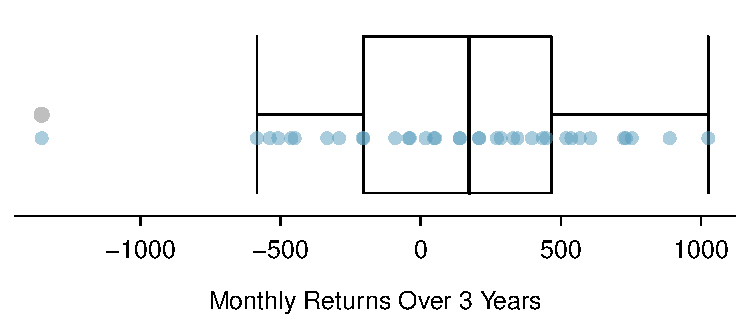
\includegraphics[width=0.6\textwidth]{ch_probability/figures/changeInLeonardsStockPortfolioFor36Months/changeInLeonardsStockPortfolioFor36Months}
\caption{The change in a portfolio like Leonard's for 36 months,
    where \$6000 is in Caterpillar's stock and \$2000 is in
    Exxon Mobil's.}
\label{changeInLeonardsStockPortfolioFor36Months}
\end{figure}

Just as we have done in many previous cases,
we use the variance and standard deviation to describe
the uncertainty associated with Leonard's monthly returns.
To do so, the variances of each stock's monthly return
will be useful, and these are shown in
Figure~\ref{sumStatOfCATXOM}.
The stocks' returns are nearly independent.

\begin{figure}
\centering
\begin{tabular}{lrrr}
\hline
    & Mean ($\bar{x}$) & Standard deviation ($s$) &
	    Variance ($s^2$) \\
\hline
CAT & 0.0204  & 0.0757  & 0.0057 \\
XOM & 0.0025  & 0.0455  & 0.0021 \\
\hline
\end{tabular}
\caption{The mean, standard deviation, and variance of the
    CAT and XOM stocks.
    These statistics were estimated from historical
    stock data, so notation used for sample statistics
    has been used.}
\label{sumStatOfCATXOM}
\end{figure}

Here we use an equation from probability theory to
describe the uncertainty of Leonard's monthly returns;
we leave the proof of this method to a dedicated
probability course.
The variance of a linear combination of random variables
can be computed by plugging in the variances of the
individual random variables and squaring the coefficients
of the random variables:
\begin{align*}
Var(aX + bY) = a^2\times Var(X) + b^2\times Var(Y)
\end{align*}
It is important to note that this equality assumes the
random variables are independent;
%\Comment{new description here about if independence is broken}
if independence doesn't hold, then a modification to
this equation would be required that we leave as a topic
for a future course to cover.
This equation can be used to compute the variance of
Leonard's monthly return:
\begin{align*}
Var(6000\times X + 2000\times Y)
	&= 6000^2\times Var(X) + 2000^2\times Var(Y) \\
	&= 36,000,000\times 0.0057 + 4,000,000\times 0.0021 \\
	&\approx 213,600
% sum(c(36e6, 4e6) * c(0.0057, 0.0021))
\end{align*}
The standard deviation is computed as the square root
of the variance: $\sqrt{213,600} = \$463$.
While an average monthly return of \$124 on an
\$8000 investment is nothing to scoff at,
the monthly returns are so volatile that Leonard should
not expect this income to be very stable.

\begin{onebox}{Variability of linear combinations of random variables}
The variance of a linear combination of random variables may be computed by squaring the constants, substituting in the variances for the random variables, and computing the result:
\begin{align*}
Var(aX + bY) = a^2\times Var(X) + b^2\times Var(Y)
\end{align*}
This equation is valid as long as the random variables are independent of each other. The standard deviation of the linear combination may be found by taking the square root of the variance.
\end{onebox}

\begin{examplewrap}
\begin{nexample}{Suppose John's daily commute has a standard deviation of 4 minutes. What is the uncertainty in his total commute time for the week?} \label{sdOfJohnsCommuteWeeklyTime}
The expression for John's commute time was
\begin{align*}
X_1 + X_2 + X_3 + X_4 + X_5
\end{align*}
Each coefficient is 1, and the variance of each day's time is $4^2=16$. Thus, the variance of the total weekly commute time is
\begin{align*}
&\text{variance }= 1^2 \times  16 + 1^2 \times  16 + 1^2 \times  16 + 1^2 \times  16 + 1^2 \times  16 = 5\times 16 = 80 \\
&\text{standard deviation } = \sqrt{\text{variance}} = \sqrt{80} = 8.94
\end{align*}
The standard deviation for John's weekly work commute time is about 9 minutes.
\end{nexample}
\end{examplewrap}

\begin{exercisewrap}
\begin{nexercise}
The computation in Example~\ref{sdOfJohnsCommuteWeeklyTime} relied on an important assumption: the commute time for each day is independent of the time on other days of that week. Do you think this is valid? Explain.\footnotemark
\end{nexercise}
\end{exercisewrap}
\footnotetext{One concern is whether traffic patterns tend to have a weekly cycle (e.g. Fridays may be worse than other days). If that is the case, and John drives, then the assumption is probably not reasonable. However, if John walks to work, then his commute is probably not affected by any weekly traffic cycle.}

\begin{exercisewrap}
\begin{nexercise}\label{elenaIsSellingATVAndBuyingAToasterOvenAtAnAuctionVariability}
Consider Elena's two auctions from Guided Practice~\ref{elenaIsSellingATVAndBuyingAToasterOvenAtAnAuction} on page~\pageref{elenaIsSellingATVAndBuyingAToasterOvenAtAnAuction}. Suppose these auctions are approximately independent and the variability in auction prices associated with the TV and toaster oven can be described using standard deviations of \$25 and \$8. Compute the standard deviation of Elena's net gain.\footnotemark
\end{nexercise}
\end{exercisewrap}
\footnotetext{The equation for Elena can be written as
\begin{align*}
(1)\times X + (-1)\times Y
\end{align*}
The variances of $X$ and $Y$ are 625 and 64. We square the coefficients and plug in the variances:
\begin{align*}
(1)^2\times Var(X) + (-1)^2\times Var(Y) = 1\times 625 + 1\times 64 = 689
\end{align*}
The variance of the linear combination is 689, and the standard deviation is the square root of 689: about \$26.25.}

Consider again Guided Practice~\ref{elenaIsSellingATVAndBuyingAToasterOvenAtAnAuctionVariability}. The negative coefficient for $Y$ in the linear combination was eliminated when we squared the coefficients. This generally holds true: negatives in a linear combination will have no impact on the variability computed for a linear combination, but they do impact the expected value computations.

\index{random variable|)}


{\exercisesheader{}

% 1

\eoce{\qt{College smokers\label{college_smokers}} At a university, 13\% of 
students smoke.
\begin{parts}
\item Calculate the expected number of smokers in a random sample of 100 students 
from this university.
\item The university gym opens at 9 am on Saturday mornings. One Saturday morning 
at 8:55 am there are 27 students outside the gym waiting for it to open. Should 
you use the same approach from part (a) to calculate the expected number of 
smokers among these 27 students?
\end{parts}
}{}

% 2

\eoce{\qt{Ace of clubs wins\label{ace_of_clubs}} Consider the following card game 
with a well-shuffled deck of cards. If you draw a red card, you win nothing. If 
you get a spade, you win \$5. For any club, you win \$10 plus an extra \$20 for 
the ace of clubs.
\begin{parts}
\item Create a probability model for the amount you win at this game. Also, find 
the expected winnings for a single game and the standard deviation of the 
winnings.
\item What is the maximum amount you would be willing to pay to play this game? 
Explain your reasoning.
\end{parts}
}{}

% 3

\eoce{\qt{Hearts win\label{hearts}} In a new card game, you start
with a well-shuffled full deck and draw 3 cards without replacement.
If you draw 3 hearts, 
you win \$50. If you draw 3 black cards, you win \$25. For any other draws, you 
win nothing.
\begin{parts}
\item Create a probability model for the amount you win at this game, and find 
the expected winnings. Also compute the standard deviation of this distribution.
\item If the game costs \$5 to play, what would be the expected value and 
standard deviation of the net profit (or loss)? \textit{(Hint: 
profit = winnings $-$ cost; $X-5$)}
\item If the game costs \$5 to play, should you play this game? Explain.
\end{parts}
}{}

% 4

\eoce{\qtq{Is it worth it\label{worth_it}} Andy is always looking for ways to 
make money fast. Lately, he has been trying to make money by gambling. Here is 
the game he is considering playing: The game costs \$2 to play. He draws a card 
from a deck. If he gets a number card (2-10), he wins nothing. For any face card (
jack, queen or king), he wins \$3. For any ace, he wins \$5, and he wins an 
\textit{extra} \$20 if he draws the ace of clubs.
\begin{parts}
\item Create a probability model and find Andy's expected profit per game.
\item Would you recommend this game to Andy as a good way to make money? Explain.
\end{parts}
}{}

% 5

\eoce{\qt{Portfolio return\label{portfolio_return}} A portfolio's value increases 
by 18\% during a financial boom and by 9\% during normal times. It decreases by 
12\% during a recession. What is the expected return on this portfolio if each 
scenario is equally likely?
}{}

% 6

\eoce{\qt{Baggage fees\label{baggage_fees}} An airline charges the following 
baggage fees: \$25 for the first bag and \$35 for the second. Suppose 54\% of 
passengers have no checked luggage, 34\% have one piece of checked luggage and 
12\% have two pieces. We suppose a negligible portion of people check more than 
two bags.
\begin{parts}
\item Build a probability model, compute the average revenue per passenger, and 
compute the corresponding standard deviation.
\item About how much revenue should the airline expect for a flight of 120 
passengers? With what standard deviation? Note any assumptions you make and if 
you think they are justified.
\end{parts}
}{}

% 7

\eoce{\qt{American roulette\label{roulette_american}} The game of American 
roulette involves spinning a wheel with 38 slots: 18 red, 18 black, and 2 green. 
A ball is spun onto the wheel and will eventually land in a slot, where each slot 
has an equal chance of capturing the ball. Gamblers can place bets on red or 
black. If the ball lands on their color, they double their money. If it lands on 
another color, they lose their money. Suppose you bet \$1 on red. What's the 
expected value and standard deviation of your winnings?
}{}

% 8

\eoce{\qt{European roulette\label{roulette_european}} The game of European 
roulette involves spinning a wheel with 37 slots: 18 red, 18 black, and 1 green. 
A ball is spun onto the wheel and will eventually land in a slot, where each slot 
has an equal chance of capturing the ball. Gamblers can place bets on red or 
black. If the ball lands on their color, they double their money. If it lands on 
another color, they lose their money.
\begin{parts}
\item Suppose you play roulette and bet \$3 on a single round. What is the 
expected value and standard deviation of your total winnings?
\item Suppose you bet \$1 in three different rounds. What is the expected value 
and standard deviation of your total winnings?
\item How do your answers to parts (a) and (b) compare? What does this say about 
the riskiness of the two games?
\end{parts}
}{}
}





%_________________
\section{Continuous distributions}
\label{contDist}

\index{data!US adult heights|(}
\index{hollow histogram|(}
\begin{examplewrap}
\begin{nexample}{Figure~\ref{fdicHistograms} shows a few
    different hollow histograms for the heights of US adults.
    How does changing the number of bins allow you to make
    different interpretations of the data?}
  \label{usHeights}%
  Adding more bins provides greater detail.
  This sample is extremely large, which is why much smaller
  bins still work well.
  Usually we do not use so many bins with smaller sample
  sizes since small counts per bin mean the bin heights
  are very volatile.
\end{nexample}
\end{examplewrap}

\begin{figure}[ht]
  \centering
  \Figure{}{fdicHistograms}
  \caption{Four hollow histograms of US adults heights
      with varying bin widths.}
  \label{fdicHistograms}
\end{figure}

\begin{examplewrap}
\begin{nexample}{What proportion of the sample is between \resp{180} cm and \resp{185} cm tall (about 5'11" to 6'1")?}\label{contDistProb}
We can add up the heights of the bins in the range \resp{180} cm and \resp{185} and divide by the sample size. For instance, this can be done with the two shaded bins shown in Figure~\ref{usHeightsHist180185}. The two bins in this region have counts of 195,307 and 156,239 people, resulting in the following estimate of the probability:
\begin{align*}
\frac{195307 + 156239}{\text{3,000,000}} = 0.1172
\end{align*}
This fraction is the same as the proportion of the histogram's area that falls in the range \resp{180} to \resp{185} cm.
\end{nexample}
\end{examplewrap}

\begin{figure}[h]
  \centering
  \Figure{0.9}{usHeightsHist180185}
  \caption{A histogram with bin sizes of 2.5 cm.
      The shaded region represents individuals with
      heights between \resp{180} and \resp{185} cm.}
  \label{usHeightsHist180185}
\end{figure}


\D{\newpage}

\subsection{From histograms to continuous distributions}

Examine the transition from a boxy hollow histogram in the top-left of Figure~\ref{fdicHistograms} to the much smoother plot in the lower-right. In this last plot, the bins are so slim that the hollow histogram is starting to resemble a smooth curve. This suggests the population height as a \emph{continuous} numerical variable might best be explained by a curve that represents the outline of extremely slim bins.

This smooth curve represents a \term{probability density function} (also called a \term{density} or \term{distribution}), and such a curve is shown in Figure~\ref{fdicHeightContDist} overlaid on a histogram of the sample. A density has a special property: the total area under the density's curve is 1. 

\begin{figure}[tbh]
\centering
\includegraphics[width=0.9\textwidth]{ch_probability/figures/fdicHeightContDist/fdicHeightContDist}
\caption{The continuous probability distribution of heights for US adults.}
\label{fdicHeightContDist}
\end{figure}

\index{hollow histogram|)}


\D{\newpage}

\subsection{Probabilities from continuous distributions}

We computed the proportion of individuals with heights \resp{180} to \resp{185} cm in Example~\ref{contDistProb} as a fraction:
\begin{align*}
\frac{\text{number of people between \resp{180} and \resp{185}}}{\text{total sample size}}
\end{align*}
We found the number of people with heights between \resp{180} and \resp{185} cm by determining the fraction of the histogram's area in this region. Similarly, we can use the area in the shaded region under the curve to find a probability (with the help of a computer):
\begin{align*}
P(\text{\var{height} between \resp{180} and \resp{185}})
	= \text{area between \resp{180} and \resp{185}}
	= 0.1157
\end{align*}
The probability that a randomly selected person is between \resp{180} and \resp{185} cm is 0.1157. This is very close to the estimate from Example~\ref{contDistProb}: 0.1172. 

\begin{figure}[h]
  \centering
  \Figure{0.7}{fdicHeightContDistFilled}
  \caption{Density for heights in the US adult population
      with the area between 180 and 185 cm shaded.
      Compare this plot with Figure~\ref{usHeightsHist180185}.}
  \label{fdicHeightContDistFilled}
\end{figure}

\begin{exercisewrap}
\begin{nexercise}
Three US adults are randomly selected. The probability a single adult is between \resp{180} and \resp{185} cm is 0.1157.\footnotemark\vspace{-1.5mm}
\begin{enumerate}
\setlength{\itemsep}{0mm}
\item[(a)] What is the probability that all three are between \resp{180} and \resp{185} cm tall?
\item[(b)] What is the probability that none are between \resp{180} and \resp{185} cm?
\end{enumerate}
\end{nexercise}
\end{exercisewrap}
\footnotetext{Brief answers:
  (a) $0.1157 \times 0.1157 \times 0.1157 = 0.0015$.
  (b) $(1-0.1157)^3 = 0.692$}

\begin{examplewrap}
\begin{nexample}{What is the probability that a randomly selected person is \textbf{exactly} \resp{180}~cm? Assume you can measure perfectly.}
\label{probabilityOfExactly180cm}
This probability is zero. A person might be close to \resp{180} cm, but not exactly \resp{180} cm tall. This also makes sense with the definition of probability as area; there is no area captured between \resp{180}~cm and \resp{180}~cm.
\end{nexample}
\end{examplewrap}

\begin{exercisewrap}
\begin{nexercise}
Suppose a person's height is rounded to the nearest centimeter. Is there a chance that a random person's \textbf{measured} height will be \resp{180} cm?\footnotemark
\end{nexercise}
\end{exercisewrap}
\footnotetext{This has positive probability. Anyone between \resp{179.5} cm and \resp{180.5} cm will have a \emph{measured} height of \resp{180} cm. This is probably a more realistic scenario to encounter in practice versus Example~\ref{probabilityOfExactly180cm}.}

\index{data!US adult heights|)}


{\exercisesheader{}

% 1

\eoce{\qt{Cat weights\label{cat_weights}} The histogram shown below represents 
the weights (in kg) of 47 female and 97 male cats. \footfullcite{cats} \\
\begin{minipage}[c]{0.47\textwidth}
\begin{parts}
\item What fraction of these cats weigh less than 2.5 kg?
\item What fraction of these cats weigh between 2.5 and 2.75 kg?
\item What fraction of these cats weigh between 2.75 and 3.5 kg?
\end{parts} \vspace{27mm}
\end{minipage}
\begin{minipage}[c]{0.05\textwidth}
$\:$ 
\end{minipage}
\begin{minipage}[c]{0.48\textwidth}
\begin{center}
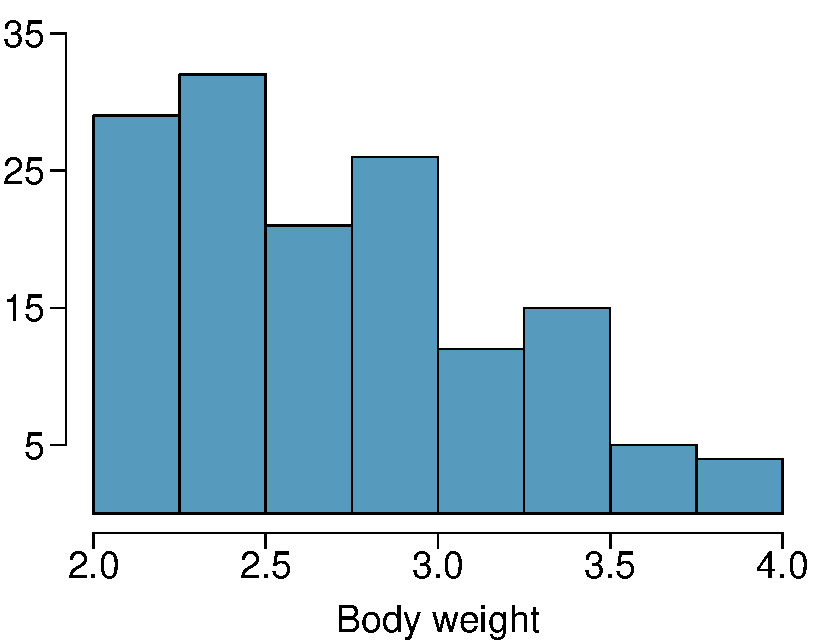
\includegraphics[width=\textwidth]{ch_probability/figures/eoce/cat_weights/cat_weights.pdf}
\end{center}
\end{minipage}
}{}

% 2

\eoce{\qt{Income and gender\label{income_gender}} The relative frequency table 
below displays the distribution of annual total personal income (in 2009 
inflation-adjusted dollars) for a representative sample of 96,420,486 Americans. 
These data come from the American Community Survey for 2005-2009. This sample is 
comprised of 59\% males and 41\% females. \footfullcite{acsIncome2005-2009} \\

\noindent\begin{minipage}[c]{0.60\textwidth}
\begin{parts}
\item Describe the distribution of total personal income.
\item What is the probability that a randomly chosen US resident makes less than 
\$50,000 per year?
\item What is the probability that a randomly chosen US resident makes less than 
\$50,000 per year and is female? Note any assumptions you make.
\item The same data source indicates that 71.8\% of females make less than 
\$50,000 per year. Use this value to determine whether or not the assumption you 
made in part (c) is valid.
\end{parts} 
\end{minipage}
\begin{minipage}[c]{0.4\textwidth}
{\small
\begin{center}
\begin{tabular}{lr}
  \hline
\textit{Income}         & \textit{Total} \\
  \hline
\$1 to \$9,999 or loss  & 2.2\% \\
\$10,000 to \$14,999    & 4.7\% \\
\$15,000 to \$24,999    & 15.8\% \\
\$25,000 to \$34,999    & 18.3\% \\
\$35,000 to \$49,999    & 21.2\% \\
\$50,000 to \$64,999    & 13.9\% \\
\$65,000 to \$74,999    & 5.8\% \\
\$75,000 to \$99,999    & 8.4\% \\
\$100,000 or more       & 9.7\% \\
   \hline
\end{tabular}
\end{center}
}
\end{minipage}
}{}
}
